% Options for packages loaded elsewhere
\PassOptionsToPackage{unicode}{hyperref}
\PassOptionsToPackage{hyphens}{url}
%
\documentclass[
]{article}
\usepackage{lmodern}
\usepackage{amsmath}
\usepackage{ifxetex,ifluatex}
\ifnum 0\ifxetex 1\fi\ifluatex 1\fi=0 % if pdftex
  \usepackage[T1]{fontenc}
  \usepackage[utf8]{inputenc}
  \usepackage{textcomp} % provide euro and other symbols
  \usepackage{amssymb}
\else % if luatex or xetex
  \usepackage{unicode-math}
  \defaultfontfeatures{Scale=MatchLowercase}
  \defaultfontfeatures[\rmfamily]{Ligatures=TeX,Scale=1}
\fi
% Use upquote if available, for straight quotes in verbatim environments
\IfFileExists{upquote.sty}{\usepackage{upquote}}{}
\IfFileExists{microtype.sty}{% use microtype if available
  \usepackage[]{microtype}
  \UseMicrotypeSet[protrusion]{basicmath} % disable protrusion for tt fonts
}{}
\makeatletter
\@ifundefined{KOMAClassName}{% if non-KOMA class
  \IfFileExists{parskip.sty}{%
    \usepackage{parskip}
  }{% else
    \setlength{\parindent}{0pt}
    \setlength{\parskip}{6pt plus 2pt minus 1pt}}
}{% if KOMA class
  \KOMAoptions{parskip=half}}
\makeatother
\usepackage{xcolor}
\IfFileExists{xurl.sty}{\usepackage{xurl}}{} % add URL line breaks if available
\IfFileExists{bookmark.sty}{\usepackage{bookmark}}{\usepackage{hyperref}}
\hypersetup{
  pdftitle={R-Bootcamp Report},
  pdfauthor={Bernardo Freire Barboza da Cruz; Leonid Gavrilyuk},
  hidelinks,
  pdfcreator={LaTeX via pandoc}}
\urlstyle{same} % disable monospaced font for URLs
\usepackage[margin=1in]{geometry}
\usepackage{longtable,booktabs}
\usepackage{calc} % for calculating minipage widths
% Correct order of tables after \paragraph or \subparagraph
\usepackage{etoolbox}
\makeatletter
\patchcmd\longtable{\par}{\if@noskipsec\mbox{}\fi\par}{}{}
\makeatother
% Allow footnotes in longtable head/foot
\IfFileExists{footnotehyper.sty}{\usepackage{footnotehyper}}{\usepackage{footnote}}
\makesavenoteenv{longtable}
\usepackage{graphicx}
\makeatletter
\def\maxwidth{\ifdim\Gin@nat@width>\linewidth\linewidth\else\Gin@nat@width\fi}
\def\maxheight{\ifdim\Gin@nat@height>\textheight\textheight\else\Gin@nat@height\fi}
\makeatother
% Scale images if necessary, so that they will not overflow the page
% margins by default, and it is still possible to overwrite the defaults
% using explicit options in \includegraphics[width, height, ...]{}
\setkeys{Gin}{width=\maxwidth,height=\maxheight,keepaspectratio}
% Set default figure placement to htbp
\makeatletter
\def\fps@figure{htbp}
\makeatother
\setlength{\emergencystretch}{3em} % prevent overfull lines
\providecommand{\tightlist}{%
  \setlength{\itemsep}{0pt}\setlength{\parskip}{0pt}}
\setcounter{secnumdepth}{5}
\ifluatex
  \usepackage{selnolig}  % disable illegal ligatures
\fi

\title{R-Bootcamp Report}
\author{Bernardo Freire Barboza da Cruz\footnote{Hochschule Luzern,
  \href{mailto:bernardo.dacruz@stud.hslu.ch}{\nolinkurl{bernardo.dacruz@stud.hslu.ch}}} \and Leonid
Gavrilyuk\footnote{Hochschule Luzern,
  \href{mailto:leonid.gavrilyuk@stud.hslu.ch}{\nolinkurl{leonid.gavrilyuk@stud.hslu.ch}}}}
\date{18 February, 2022}

\begin{document}
\maketitle

\centering
\raggedright
\newpage
\tableofcontents
\pagebreak

\hypertarget{introduction.}{%
\section{Introduction.}\label{introduction.}}

\hypertarget{project-goal}{%
\subsection{Project goal}\label{project-goal}}

The goal is to understand the dynamics in the performance of each part
in each electoral district of the city. The time span in interest is
\textbf{2006-2018 ???} The questions to be answered: the portrait of the
voters, identification of relationship (if any) between such
characteristics as voters' education or age and the election results of
the party.

\hypertarget{data}{%
\subsection{Data}\label{data}}

To perform analysis, six data sets covering the time period 2006-2022
were retrieved from the Open Data platform of the City of Zürich:

\begin{itemize}
\tightlist
\item
  Turnout at the city and municipal council elections, by city district,
  since 2006. (\emph{Beteiligung am Urnengang der Stadt- und
  Gemeinderatswahlen nach Stadtquartier})
\item
  Municipal elections vote share, by party and electoral district, since
  1913. (\emph{Gemeinderatswahlen Stimmenanteil nach Partei und
  Wahlkreis})
\item
  Turnout at the city and municipal council elections, by age and
  gender, since 2006. ?? ??
\end{itemize}

The data sets did not have the same content and were not organised in
the same way. Each data set contained some irrelevant information - for
example, historical election data since 1913 whereas the time span of
interest is 2006-2018. This required data preparation activities. Each
data set was prepared, subsequently all of them were merged into one
final table.

\pagebreak

\hypertarget{data-preparation}{%
\section{Data Preparation}\label{data-preparation}}

\hypertarget{data-set-1-turnout-at-the-city-and-municipal-council-elections-since-2006-by-city-district.}{%
\subsection{Data set 1: Turnout at the city and municipal council
elections since 2006, by city
district.}\label{data-set-1-turnout-at-the-city-and-municipal-council-elections-since-2006-by-city-district.}}

The data set of dimensions 136x7 reflects how many people from each city
district participated in five last elections (2006-2022).

\begin{longtable}[]{@{}rrlrrrr@{}}
\caption{Original data set: Turnout in the city and municipal council
elections since 2006, by city district}\tabularnewline
\toprule
Jahr & QNr & Qname & Sberechtigte & Nteilnehmende & teilnehmende &
Beteiligung\tabularnewline
\midrule
\endfirsthead
\toprule
Jahr & QNr & Qname & Sberechtigte & Nteilnehmende & teilnehmende &
Beteiligung\tabularnewline
\midrule
\endhead
2006 & 11 & Rathaus (Kreis 1) & 1974 & 1186 & 788 & 39.9\tabularnewline
2006 & 12 & Hochschulen (Kreis 1) & 377 & 232 & 145 &
38.5\tabularnewline
2006 & 13 & Lindenhof (Kreis 1) & 1335 & 962 & 373 & 27.9\tabularnewline
2006 & 14 & City (Kreis 1) & 597 & 440 & 157 & 26.3\tabularnewline
2006 & 21 & Wollishofen (Kreis 2) & 10115 & 6168 & 3947 &
39.0\tabularnewline
2006 & 23 & Leimbach (Kreis 2) & 3123 & 1997 & 1126 &
36.1\tabularnewline
\bottomrule
\end{longtable}

Examination of the dataset revealed an important issue: The territorial
entity in this dataset is a city district - \emph{``Stadtquartier''}.
However, in Zürich, the elections are held across 12 electoral districts
- \emph{``Wahlkreise''}. Each electoral district consists of several
``Stadtquartiers''. For example, electoral district ``Kreis 1+2'' unites
six city districts (they are shown in the ``Qname'' column in the Table
1 above).

To address the issue, the following manipulations were performed:

\begin{itemize}
\tightlist
\item
  In the column ``Qname'', the electoral district is specified in the
  parentheses: e.g.~``Rathaus (Kreis 1)''. The content of the
  parentheses was extracted with the \textbf{stringr package} and stored
  in the created column ``DistrictName''.
\item
  Rename the electoral districts to reflect the fact that some city
  districts are merged for the elections - for example ``Kreis 1'' and
  ``Kreis 2'' became ``Kreis 1+2''. This was done with the \textbf{dplyr
  mutate() function}.
\item
  Calculate the mean values for each group and year using \textbf{dplyr
  group\_by() and summarise() functions} (saved as a separate data
  frame). The results is saved as a separate data frame, with the new
  column ``PercentageOfDistrict''.
\item
  Calculate percentage of each district's voters relative to the total
  number of the city voters using \textbf{dplyr group\_by()
  \%\textgreater\% summarise() \%\textgreater\% transmute() functions}.
  The results is saved as a separate data frame, with the new column
  ``PercentageOfCity''.
\item
  Merge the dataframes with the \textbf{dplyr inner\_join()}.
\item
  Change ``Jahr'' and ``DistrictName'' to factors with the built-in
  \textbf{as.factor()}
\end{itemize}

\begin{longtable}[]{@{}llrr@{}}
\caption{Final dataset: Turnout by electoral district}\tabularnewline
\toprule
Jahr & DistrictName & PercentageOfDistrict &
PercentageOfCity\tabularnewline
\midrule
\endfirsthead
\toprule
Jahr & DistrictName & PercentageOfDistrict &
PercentageOfCity\tabularnewline
\midrule
\endhead
2006 & Kreis 1+2 & 34.95714 & 11.436022\tabularnewline
2006 & Kreis 10 & 38.25000 & 12.176240\tabularnewline
2006 & Kreis 11 & 31.80000 & 13.336140\tabularnewline
2006 & Kreis 12 & 29.56667 & 5.654176\tabularnewline
2006 & Kreis 3 & 33.20000 & 11.112771\tabularnewline
2006 & Kreis 4+5 & 28.20000 & 7.482310\tabularnewline
\bottomrule
\end{longtable}

The analysis shows that the amount of voters in each district has grown
since 2006 - Zürich residents are becoming more active in exercising
their right to vote. Kreis 6 has the highest percentage of active
citizens, followed by Kreis 7+8 and Kreis 10. Residents of Kreis 12 are
the least interested in the elections people in Zürich. However, when it
comes to the percentage of all city voters, Kreis 12 contributes the
third largest portion of votes. This means, politicians should mobilize
residents of this district to gain votes on the city and national level
elections. Other important districts are Kreis 7+8 (gives most votes)
and Kreis 11 (second place).

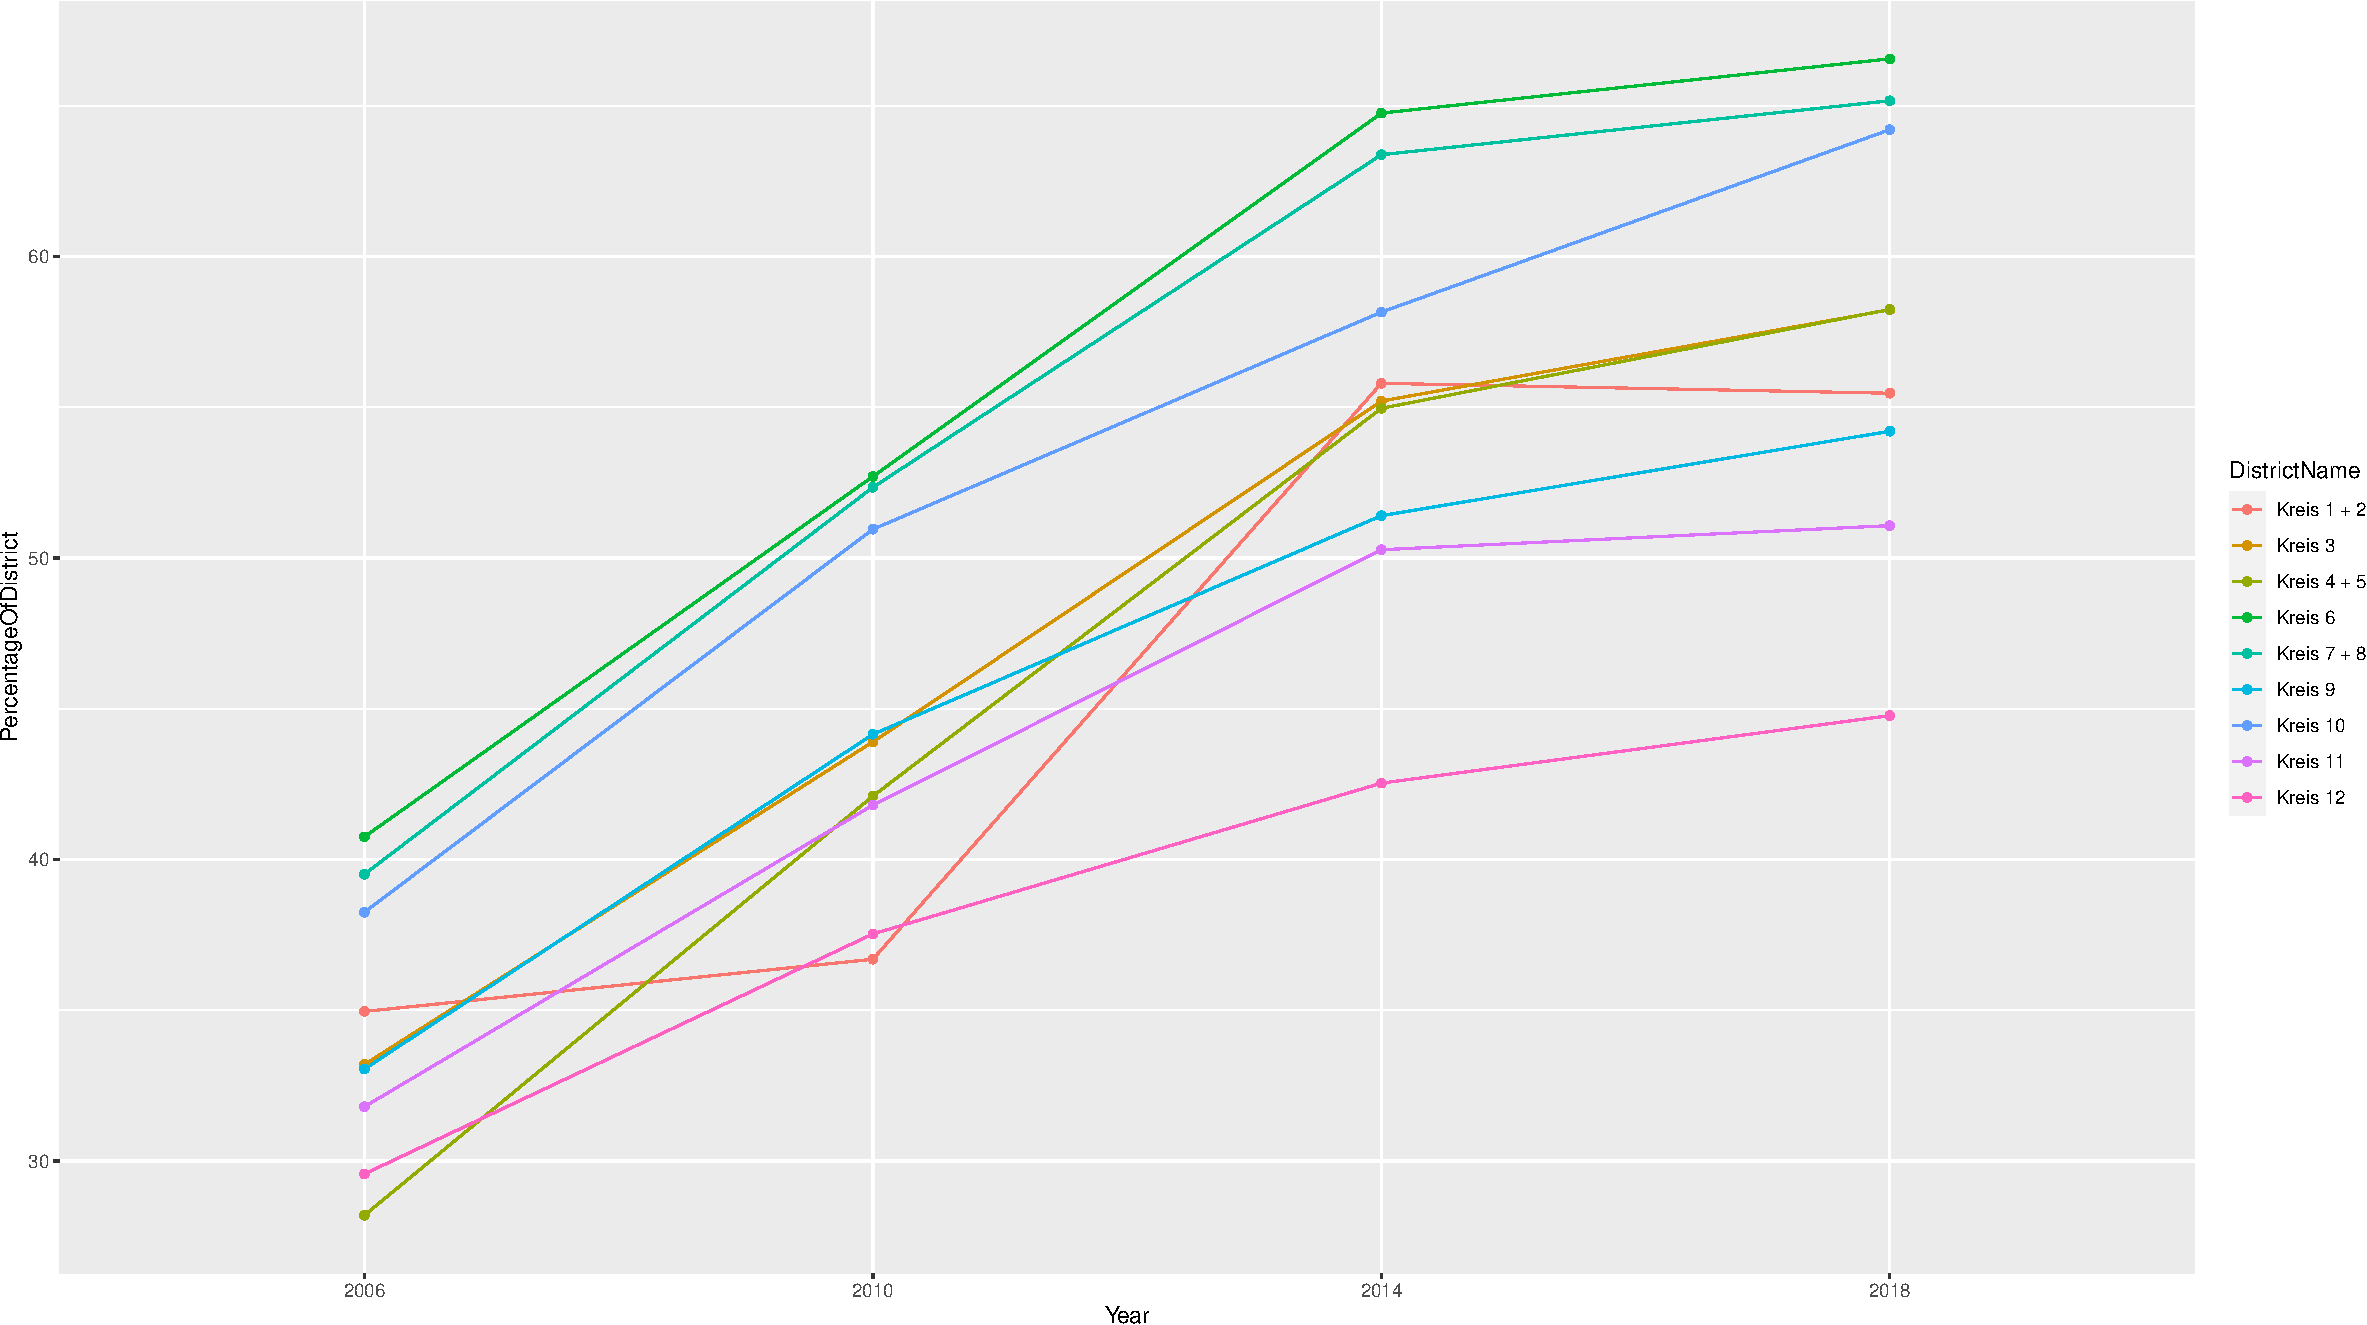
\includegraphics{report_files/figure-latex/plot_election_per_district-1.pdf}

\hypertarget{data-set-2-municipal-elections-vote-share-by-party-and-electoral-district-since-1913.}{%
\subsection{Data set 2: Municipal elections vote share, by party and
electoral district since
1913.}\label{data-set-2-municipal-elections-vote-share-by-party-and-electoral-district-since-1913.}}

The data set of dimensions 5100x6 shows the results of each party at the
elections since 1913. Naturally, it contains a lot of irrelevant
information because of the changes that happened sine 1913. For example,
for each year there are separate rows for ``Kreis 1 (before 2002)'',
``Kreis 2 (before 2002) and''Kreis 1+2 (after 2006)" - the districts
were united in 2002. Some political parties do not exist anymore; some
parties changed their names. Additionally, the table is in the long
format whereas the final data set requires it to be wide.

\begin{longtable}[]{@{}rlrlrr@{}}
\caption{Original data set: Municipal elections vote share, by party and
electoral district since 1913.}\tabularnewline
\toprule
Jahr & Partei & ParteiNr & Wahlkreis & WahlkreisSort &
Stimmenanteil\tabularnewline
\midrule
\endfirsthead
\toprule
Jahr & Partei & ParteiNr & Wahlkreis & WahlkreisSort &
Stimmenanteil\tabularnewline
\midrule
\endhead
1913 & SP & 1 & Stadt Zürich & 0 & 39.1\tabularnewline
1913 & BGB/SVP & 2 & Stadt Zürich & 0 & NA\tabularnewline
1913 & FDP & 3 & Stadt Zürich & 0 & 38.6\tabularnewline
1913 & GPS & 4 & Stadt Zürich & 0 & NA\tabularnewline
1913 & GLP & 5 & Stadt Zürich & 0 & NA\tabularnewline
1913 & CVP/Die Mitte & 6 & Stadt Zürich & 0 & 7.9\tabularnewline
\bottomrule
\end{longtable}

The following manipulations were performed:

\begin{itemize}
\tightlist
\item
  Choose only relevant time period (years 2006-2018) and eight still
  existing parties using the \textbf{\%in\% operator}.
\item
  Change the names of the electoral districts. For example, ``Kreis 11
  (ab 1974)'' became simply ``Kreis 11'' - the content in the
  parentheses was removed with the \textbf{stringr str\_replace()
  function}.
\item
  Rename the columns with the \textbf{dplyr \%\textgreater\% rename()
  function} to keep them in line with the other tables
  (e.g.~``Wahlkreis'' to ``DistrictName'').
\item
  Remove unnecessary columns with the \textbf{dplyr \%\textgreater\%
  select() function}.
\item
  Transform the table into wide format with the \textbf{tidyverse
  pivot\_wider() function}.
\item
  Merge the set with the first table ``Turnout by electoral district''
  (see part 2.1.)
\end{itemize}

\begin{longtable}[]{@{}rlrrrrrrrr@{}}
\caption{Final dataset: Municipal elections vote share, by party and
electoral district, 2006-2018.}\tabularnewline
\toprule
Year & DistrictName & SP & BGB/SVP & FDP & GPS & GLP & CVP/Die Mitte &
AL & EVP\tabularnewline
\midrule
\endfirsthead
\toprule
Year & DistrictName & SP & BGB/SVP & FDP & GPS & GLP & CVP/Die Mitte &
AL & EVP\tabularnewline
\midrule
\endhead
2006 & Kreis 1 + 2 & 30.1 & 16.2 & 23.1 & 13.1 & 2.4 & 7.7 & 2.5 &
3.0\tabularnewline
2010 & Kreis 1 + 2 & 28.0 & 16.9 & 19.3 & 13.7 & 8.6 & 5.8 & 2.6 &
1.9\tabularnewline
2014 & Kreis 1 + 2 & 26.6 & 16.2 & 21.0 & 11.4 & 10.5 & 5.1 & 4.9 &
1.9\tabularnewline
2018 & Kreis 1 + 2 & 30.8 & 13.1 & 19.8 & 12.4 & 10.4 & 4.3 & 6.3 &
1.5\tabularnewline
2006 & Kreis 3 & 37.5 & 18.2 & 8.6 & 14.3 & 2.3 & 7.1 & 6.1 &
2.3\tabularnewline
2010 & Kreis 3 & 34.2 & 16.9 & 8.1 & 13.5 & 10.4 & 5.1 & 6.9 &
1.7\tabularnewline
2014 & Kreis 3 & 32.1 & 15.0 & 10.5 & 12.8 & 10.4 & 4.0 & 9.8 &
1.4\tabularnewline
2018 & Kreis 3 & 35.8 & 10.3 & 10.9 & 14.1 & 10.4 & 3.2 & 12.1 &
1.6\tabularnewline
\bottomrule
\end{longtable}

The analysis shows that

\hypertarget{data-set-3-wealth-distribution-of-the-population-in-zuxfcrich-by-district}{%
\subsection{Data set 3: Wealth distribution of the population in Zürich,
by
district}\label{data-set-3-wealth-distribution-of-the-population-in-zuxfcrich-by-district}}

The data set of dimensions 756x8 variables reflects how the wealth
distribution in absolute terms changed over time per district and per
tax class. The following table shows the accumulated wealth distribution
across all districts of the city of Zürich between the years 1999 and
2019.

\begin{longtable}[]{@{}rrlr@{}}
\caption{Original data set: Distribution wealth tax per category,
district and year}\tabularnewline
\toprule
SteuerJahr & KreisSort & KreisLang & SteuerTarifSort\tabularnewline
\midrule
\endfirsthead
\toprule
SteuerJahr & KreisSort & KreisLang & SteuerTarifSort\tabularnewline
\midrule
\endhead
1999 & 1 & Kreis 1 & 0\tabularnewline
1999 & 1 & Kreis 1 & 1\tabularnewline
1999 & 1 & Kreis 1 & 2\tabularnewline
1999 & 2 & Kreis 2 & 0\tabularnewline
1999 & 2 & Kreis 2 & 1\tabularnewline
1999 & 2 & Kreis 2 & 2\tabularnewline
\bottomrule
\end{longtable}

\begin{longtable}[]{@{}rlrrr@{}}
\toprule
\begin{minipage}[b]{(\columnwidth - 4\tabcolsep) * \real{0.16}}\raggedleft
SteuerTarifSort\strut
\end{minipage} &
\begin{minipage}[b]{(\columnwidth - 4\tabcolsep) * \real{0.23}}\raggedright
SteuerTarifLang\strut
\end{minipage} &
\begin{minipage}[b]{(\columnwidth - 4\tabcolsep) * \real{0.20}}\raggedleft
SteuerVermoegen\_p50\strut
\end{minipage} &
\begin{minipage}[b]{(\columnwidth - 4\tabcolsep) * \real{0.20}}\raggedleft
SteuerVermoegen\_p25\strut
\end{minipage} &
\begin{minipage}[b]{(\columnwidth - 4\tabcolsep) * \real{0.20}}\raggedleft
SteuerVermoegen\_p75\strut
\end{minipage}\tabularnewline
\midrule
\endhead
\begin{minipage}[t]{(\columnwidth - 4\tabcolsep) * \real{0.16}}\raggedleft
0\strut
\end{minipage} &
\begin{minipage}[t]{(\columnwidth - 4\tabcolsep) * \real{0.23}}\raggedright
Grundtarif\strut
\end{minipage} &
\begin{minipage}[t]{(\columnwidth - 4\tabcolsep) * \real{0.20}}\raggedleft
23.0\strut
\end{minipage} &
\begin{minipage}[t]{(\columnwidth - 4\tabcolsep) * \real{0.20}}\raggedleft
0\strut
\end{minipage} &
\begin{minipage}[t]{(\columnwidth - 4\tabcolsep) * \real{0.20}}\raggedleft
174\strut
\end{minipage}\tabularnewline
\begin{minipage}[t]{(\columnwidth - 4\tabcolsep) * \real{0.16}}\raggedleft
1\strut
\end{minipage} &
\begin{minipage}[t]{(\columnwidth - 4\tabcolsep) * \real{0.23}}\raggedright
Verheiratetentarif\strut
\end{minipage} &
\begin{minipage}[t]{(\columnwidth - 4\tabcolsep) * \real{0.20}}\raggedleft
182.0\strut
\end{minipage} &
\begin{minipage}[t]{(\columnwidth - 4\tabcolsep) * \real{0.20}}\raggedleft
22\strut
\end{minipage} &
\begin{minipage}[t]{(\columnwidth - 4\tabcolsep) * \real{0.20}}\raggedleft
711\strut
\end{minipage}\tabularnewline
\begin{minipage}[t]{(\columnwidth - 4\tabcolsep) * \real{0.16}}\raggedleft
2\strut
\end{minipage} &
\begin{minipage}[t]{(\columnwidth - 4\tabcolsep) * \real{0.23}}\raggedright
Einelternfamilientarif\strut
\end{minipage} &
\begin{minipage}[t]{(\columnwidth - 4\tabcolsep) * \real{0.20}}\raggedleft
27.5\strut
\end{minipage} &
\begin{minipage}[t]{(\columnwidth - 4\tabcolsep) * \real{0.20}}\raggedleft
0\strut
\end{minipage} &
\begin{minipage}[t]{(\columnwidth - 4\tabcolsep) * \real{0.20}}\raggedleft
283\strut
\end{minipage}\tabularnewline
\begin{minipage}[t]{(\columnwidth - 4\tabcolsep) * \real{0.16}}\raggedleft
0\strut
\end{minipage} &
\begin{minipage}[t]{(\columnwidth - 4\tabcolsep) * \real{0.23}}\raggedright
Grundtarif\strut
\end{minipage} &
\begin{minipage}[t]{(\columnwidth - 4\tabcolsep) * \real{0.20}}\raggedleft
37.0\strut
\end{minipage} &
\begin{minipage}[t]{(\columnwidth - 4\tabcolsep) * \real{0.20}}\raggedleft
3\strut
\end{minipage} &
\begin{minipage}[t]{(\columnwidth - 4\tabcolsep) * \real{0.20}}\raggedleft
186\strut
\end{minipage}\tabularnewline
\begin{minipage}[t]{(\columnwidth - 4\tabcolsep) * \real{0.16}}\raggedleft
1\strut
\end{minipage} &
\begin{minipage}[t]{(\columnwidth - 4\tabcolsep) * \real{0.23}}\raggedright
Verheiratetentarif\strut
\end{minipage} &
\begin{minipage}[t]{(\columnwidth - 4\tabcolsep) * \real{0.20}}\raggedleft
148.0\strut
\end{minipage} &
\begin{minipage}[t]{(\columnwidth - 4\tabcolsep) * \real{0.20}}\raggedleft
33\strut
\end{minipage} &
\begin{minipage}[t]{(\columnwidth - 4\tabcolsep) * \real{0.20}}\raggedleft
458\strut
\end{minipage}\tabularnewline
\begin{minipage}[t]{(\columnwidth - 4\tabcolsep) * \real{0.16}}\raggedleft
2\strut
\end{minipage} &
\begin{minipage}[t]{(\columnwidth - 4\tabcolsep) * \real{0.23}}\raggedright
Einelternfamilientarif\strut
\end{minipage} &
\begin{minipage}[t]{(\columnwidth - 4\tabcolsep) * \real{0.20}}\raggedleft
7.0\strut
\end{minipage} &
\begin{minipage}[t]{(\columnwidth - 4\tabcolsep) * \real{0.20}}\raggedleft
0\strut
\end{minipage} &
\begin{minipage}[t]{(\columnwidth - 4\tabcolsep) * \real{0.20}}\raggedleft
61\strut
\end{minipage}\tabularnewline
\bottomrule
\end{longtable}

Examinating the previous showed data revealed that the data set contains
a lot of irrelevant information. For example, the columns
\emph{``KreisSort''} and \emph{``KreisLang''} are redundant, since the
first in simply the encoding of the second in number. The same applies
for the the columns \emph{``SteuerTarifSort''} and
\emph{``SteuerTarifLang''}, since the first here again, is the encoding
of the second in number. However, the columns \emph{``KreisLang''} and
\emph{``SteuerTarifLang''} are redundant and therefore, droped. For
practical reasons the columns \emph{``SteuerVermoegen\_p25''} and
\emph{``SteuerVermoegen\_p75''} were droped as well.\\
Additionally, the names of the columns do not correspond with the
previous data set and therefore, we have to change the following:

\begin{longtable}[]{@{}ll@{}}
\toprule
Original Column Name & New Column Name\tabularnewline
\midrule
\endhead
KreisSort & DistrictNumber\tabularnewline
SteuerJahr & Year\tabularnewline
SteuerVermoegen\_p50 & Wealth\tabularnewline
SteuerTarifSort & Category\tabularnewline
\bottomrule
\end{longtable}

Finally, after all modifications, the data set looks as follows:

\begin{longtable}[]{@{}rrrr@{}}
\caption{Final data set: Distribution wealth tax per category, district
and year}\tabularnewline
\toprule
Year & DistrictNumber & Category & Wealth\tabularnewline
\midrule
\endfirsthead
\toprule
Year & DistrictNumber & Category & Wealth\tabularnewline
\midrule
\endhead
1999 & 1 & 0 & 23.0\tabularnewline
1999 & 1 & 1 & 182.0\tabularnewline
1999 & 1 & 2 & 27.5\tabularnewline
1999 & 2 & 0 & 37.0\tabularnewline
1999 & 2 & 1 & 148.0\tabularnewline
1999 & 2 & 2 & 7.0\tabularnewline
1999 & 3 & 0 & 18.0\tabularnewline
1999 & 3 & 1 & 58.0\tabularnewline
1999 & 3 & 2 & 0.0\tabularnewline
1999 & 4 & 0 & 6.0\tabularnewline
1999 & 4 & 1 & 9.0\tabularnewline
1999 & 4 & 2 & 0.0\tabularnewline
1999 & 5 & 0 & 7.0\tabularnewline
1999 & 5 & 1 & 15.0\tabularnewline
1999 & 5 & 2 & 0.0\tabularnewline
1999 & 6 & 0 & 38.0\tabularnewline
1999 & 6 & 1 & 145.0\tabularnewline
1999 & 6 & 2 & 17.0\tabularnewline
1999 & 7 & 0 & 57.0\tabularnewline
1999 & 7 & 1 & 307.0\tabularnewline
1999 & 7 & 2 & 35.0\tabularnewline
1999 & 8 & 0 & 35.0\tabularnewline
1999 & 8 & 1 & 184.5\tabularnewline
1999 & 8 & 2 & 18.0\tabularnewline
1999 & 9 & 0 & 23.0\tabularnewline
1999 & 9 & 1 & 84.0\tabularnewline
1999 & 9 & 2 & 1.0\tabularnewline
1999 & 10 & 0 & 34.0\tabularnewline
1999 & 10 & 1 & 124.0\tabularnewline
1999 & 10 & 2 & 11.0\tabularnewline
1999 & 11 & 0 & 19.0\tabularnewline
1999 & 11 & 1 & 77.0\tabularnewline
1999 & 11 & 2 & 3.0\tabularnewline
1999 & 12 & 0 & 16.0\tabularnewline
1999 & 12 & 1 & 49.0\tabularnewline
1999 & 12 & 2 & 0.0\tabularnewline
2000 & 1 & 0 & 26.0\tabularnewline
2000 & 1 & 1 & 187.5\tabularnewline
2000 & 1 & 2 & 30.0\tabularnewline
2000 & 2 & 0 & 38.0\tabularnewline
2000 & 2 & 1 & 149.0\tabularnewline
2000 & 2 & 2 & 8.0\tabularnewline
2000 & 3 & 0 & 19.0\tabularnewline
2000 & 3 & 1 & 55.0\tabularnewline
2000 & 3 & 2 & 1.0\tabularnewline
2000 & 4 & 0 & 7.0\tabularnewline
2000 & 4 & 1 & 9.0\tabularnewline
2000 & 4 & 2 & 0.0\tabularnewline
2000 & 5 & 0 & 9.0\tabularnewline
2000 & 5 & 1 & 19.0\tabularnewline
2000 & 5 & 2 & 0.0\tabularnewline
2000 & 6 & 0 & 38.0\tabularnewline
2000 & 6 & 1 & 145.0\tabularnewline
2000 & 6 & 2 & 21.0\tabularnewline
2000 & 7 & 0 & 58.0\tabularnewline
2000 & 7 & 1 & 323.0\tabularnewline
2000 & 7 & 2 & 34.0\tabularnewline
2000 & 8 & 0 & 38.0\tabularnewline
2000 & 8 & 1 & 194.5\tabularnewline
2000 & 8 & 2 & 27.0\tabularnewline
2000 & 9 & 0 & 22.0\tabularnewline
2000 & 9 & 1 & 81.0\tabularnewline
2000 & 9 & 2 & 2.0\tabularnewline
2000 & 10 & 0 & 33.0\tabularnewline
2000 & 10 & 1 & 131.0\tabularnewline
2000 & 10 & 2 & 10.0\tabularnewline
2000 & 11 & 0 & 18.0\tabularnewline
2000 & 11 & 1 & 74.0\tabularnewline
2000 & 11 & 2 & 3.0\tabularnewline
2000 & 12 & 0 & 15.0\tabularnewline
2000 & 12 & 1 & 49.0\tabularnewline
2000 & 12 & 2 & 0.0\tabularnewline
2001 & 1 & 0 & 27.0\tabularnewline
2001 & 1 & 1 & 183.0\tabularnewline
2001 & 1 & 2 & 43.5\tabularnewline
2001 & 2 & 0 & 38.0\tabularnewline
2001 & 2 & 1 & 152.0\tabularnewline
2001 & 2 & 2 & 10.0\tabularnewline
2001 & 3 & 0 & 20.0\tabularnewline
2001 & 3 & 1 & 56.0\tabularnewline
2001 & 3 & 2 & 3.0\tabularnewline
2001 & 4 & 0 & 8.0\tabularnewline
2001 & 4 & 1 & 8.0\tabularnewline
2001 & 4 & 2 & 0.0\tabularnewline
2001 & 5 & 0 & 10.0\tabularnewline
2001 & 5 & 1 & 19.0\tabularnewline
2001 & 5 & 2 & 0.0\tabularnewline
2001 & 6 & 0 & 39.0\tabularnewline
2001 & 6 & 1 & 148.0\tabularnewline
2001 & 6 & 2 & 25.0\tabularnewline
2001 & 7 & 0 & 61.5\tabularnewline
2001 & 7 & 1 & 318.0\tabularnewline
2001 & 7 & 2 & 34.5\tabularnewline
2001 & 8 & 0 & 40.5\tabularnewline
2001 & 8 & 1 & 200.0\tabularnewline
2001 & 8 & 2 & 29.5\tabularnewline
2001 & 9 & 0 & 22.0\tabularnewline
2001 & 9 & 1 & 78.0\tabularnewline
2001 & 9 & 2 & 1.0\tabularnewline
2001 & 10 & 0 & 34.0\tabularnewline
2001 & 10 & 1 & 134.0\tabularnewline
2001 & 10 & 2 & 13.0\tabularnewline
2001 & 11 & 0 & 19.0\tabularnewline
2001 & 11 & 1 & 73.0\tabularnewline
2001 & 11 & 2 & 3.0\tabularnewline
2001 & 12 & 0 & 16.0\tabularnewline
2001 & 12 & 1 & 47.0\tabularnewline
2001 & 12 & 2 & 0.5\tabularnewline
2002 & 1 & 0 & 27.0\tabularnewline
2002 & 1 & 1 & 183.0\tabularnewline
2002 & 1 & 2 & 37.5\tabularnewline
2002 & 2 & 0 & 36.0\tabularnewline
2002 & 2 & 1 & 150.0\tabularnewline
2002 & 2 & 2 & 10.0\tabularnewline
2002 & 3 & 0 & 19.0\tabularnewline
2002 & 3 & 1 & 54.0\tabularnewline
2002 & 3 & 2 & 2.0\tabularnewline
2002 & 4 & 0 & 6.0\tabularnewline
2002 & 4 & 1 & 6.0\tabularnewline
2002 & 4 & 2 & 0.0\tabularnewline
2002 & 5 & 0 & 10.0\tabularnewline
2002 & 5 & 1 & 19.0\tabularnewline
2002 & 5 & 2 & 0.0\tabularnewline
2002 & 6 & 0 & 38.0\tabularnewline
2002 & 6 & 1 & 140.0\tabularnewline
2002 & 6 & 2 & 23.0\tabularnewline
2002 & 7 & 0 & 58.0\tabularnewline
2002 & 7 & 1 & 300.0\tabularnewline
2002 & 7 & 2 & 42.0\tabularnewline
2002 & 8 & 0 & 38.0\tabularnewline
2002 & 8 & 1 & 192.0\tabularnewline
2002 & 8 & 2 & 24.5\tabularnewline
2002 & 9 & 0 & 21.0\tabularnewline
2002 & 9 & 1 & 71.0\tabularnewline
2002 & 9 & 2 & 1.0\tabularnewline
2002 & 10 & 0 & 33.0\tabularnewline
2002 & 10 & 1 & 127.0\tabularnewline
2002 & 10 & 2 & 13.0\tabularnewline
2002 & 11 & 0 & 17.0\tabularnewline
2002 & 11 & 1 & 68.0\tabularnewline
2002 & 11 & 2 & 3.0\tabularnewline
2002 & 12 & 0 & 14.0\tabularnewline
2002 & 12 & 1 & 42.0\tabularnewline
2002 & 12 & 2 & 0.0\tabularnewline
2003 & 1 & 0 & 29.0\tabularnewline
2003 & 1 & 1 & 196.0\tabularnewline
2003 & 1 & 2 & 39.0\tabularnewline
2003 & 2 & 0 & 35.0\tabularnewline
2003 & 2 & 1 & 153.0\tabularnewline
2003 & 2 & 2 & 12.0\tabularnewline
2003 & 3 & 0 & 20.0\tabularnewline
2003 & 3 & 1 & 52.0\tabularnewline
2003 & 3 & 2 & 2.0\tabularnewline
2003 & 4 & 0 & 6.0\tabularnewline
2003 & 4 & 1 & 6.0\tabularnewline
2003 & 4 & 2 & 0.0\tabularnewline
2003 & 5 & 0 & 10.5\tabularnewline
2003 & 5 & 1 & 21.0\tabularnewline
2003 & 5 & 2 & 1.0\tabularnewline
2003 & 6 & 0 & 40.0\tabularnewline
2003 & 6 & 1 & 151.0\tabularnewline
2003 & 6 & 2 & 25.0\tabularnewline
2003 & 7 & 0 & 60.0\tabularnewline
2003 & 7 & 1 & 326.0\tabularnewline
2003 & 7 & 2 & 41.0\tabularnewline
2003 & 8 & 0 & 41.0\tabularnewline
2003 & 8 & 1 & 198.5\tabularnewline
2003 & 8 & 2 & 31.0\tabularnewline
2003 & 9 & 0 & 21.0\tabularnewline
2003 & 9 & 1 & 73.0\tabularnewline
2003 & 9 & 2 & 2.0\tabularnewline
2003 & 10 & 0 & 33.0\tabularnewline
2003 & 10 & 1 & 140.0\tabularnewline
2003 & 10 & 2 & 13.5\tabularnewline
2003 & 11 & 0 & 18.0\tabularnewline
2003 & 11 & 1 & 69.0\tabularnewline
2003 & 11 & 2 & 2.0\tabularnewline
2003 & 12 & 0 & 14.0\tabularnewline
2003 & 12 & 1 & 42.0\tabularnewline
2003 & 12 & 2 & 0.0\tabularnewline
2004 & 1 & 0 & 27.0\tabularnewline
2004 & 1 & 1 & 199.0\tabularnewline
2004 & 1 & 2 & 65.0\tabularnewline
2004 & 2 & 0 & 35.0\tabularnewline
2004 & 2 & 1 & 152.0\tabularnewline
2004 & 2 & 2 & 13.0\tabularnewline
2004 & 3 & 0 & 20.0\tabularnewline
2004 & 3 & 1 & 52.0\tabularnewline
2004 & 3 & 2 & 2.5\tabularnewline
2004 & 4 & 0 & 6.0\tabularnewline
2004 & 4 & 1 & 4.0\tabularnewline
2004 & 4 & 2 & 0.0\tabularnewline
2004 & 5 & 0 & 13.0\tabularnewline
2004 & 5 & 1 & 20.0\tabularnewline
2004 & 5 & 2 & 2.0\tabularnewline
2004 & 6 & 0 & 41.0\tabularnewline
2004 & 6 & 1 & 152.0\tabularnewline
2004 & 6 & 2 & 25.0\tabularnewline
2004 & 7 & 0 & 61.0\tabularnewline
2004 & 7 & 1 & 337.0\tabularnewline
2004 & 7 & 2 & 42.0\tabularnewline
2004 & 8 & 0 & 40.0\tabularnewline
2004 & 8 & 1 & 201.0\tabularnewline
2004 & 8 & 2 & 36.0\tabularnewline
2004 & 9 & 0 & 20.0\tabularnewline
2004 & 9 & 1 & 69.0\tabularnewline
2004 & 9 & 2 & 1.0\tabularnewline
2004 & 10 & 0 & 34.0\tabularnewline
2004 & 10 & 1 & 144.0\tabularnewline
2004 & 10 & 2 & 13.0\tabularnewline
2004 & 11 & 0 & 18.0\tabularnewline
2004 & 11 & 1 & 66.0\tabularnewline
2004 & 11 & 2 & 3.0\tabularnewline
2004 & 12 & 0 & 13.0\tabularnewline
2004 & 12 & 1 & 37.0\tabularnewline
2004 & 12 & 2 & 0.0\tabularnewline
2005 & 1 & 0 & 34.0\tabularnewline
2005 & 1 & 1 & 234.0\tabularnewline
2005 & 1 & 2 & 28.0\tabularnewline
2005 & 2 & 0 & 37.0\tabularnewline
2005 & 2 & 1 & 162.0\tabularnewline
2005 & 2 & 2 & 14.0\tabularnewline
2005 & 3 & 0 & 20.0\tabularnewline
2005 & 3 & 1 & 53.0\tabularnewline
2005 & 3 & 2 & 3.0\tabularnewline
2005 & 4 & 0 & 7.0\tabularnewline
2005 & 4 & 1 & 3.0\tabularnewline
2005 & 4 & 2 & 0.0\tabularnewline
2005 & 5 & 0 & 15.0\tabularnewline
2005 & 5 & 1 & 20.0\tabularnewline
2005 & 5 & 2 & 4.0\tabularnewline
2005 & 6 & 0 & 43.0\tabularnewline
2005 & 6 & 1 & 164.0\tabularnewline
2005 & 6 & 2 & 27.0\tabularnewline
2005 & 7 & 0 & 62.0\tabularnewline
2005 & 7 & 1 & 352.0\tabularnewline
2005 & 7 & 2 & 44.0\tabularnewline
2005 & 8 & 0 & 43.0\tabularnewline
2005 & 8 & 1 & 218.0\tabularnewline
2005 & 8 & 2 & 27.0\tabularnewline
2005 & 9 & 0 & 19.0\tabularnewline
2005 & 9 & 1 & 67.0\tabularnewline
2005 & 9 & 2 & 1.0\tabularnewline
2005 & 10 & 0 & 34.0\tabularnewline
2005 & 10 & 1 & 147.0\tabularnewline
2005 & 10 & 2 & 16.5\tabularnewline
2005 & 11 & 0 & 17.0\tabularnewline
2005 & 11 & 1 & 65.0\tabularnewline
2005 & 11 & 2 & 2.0\tabularnewline
2005 & 12 & 0 & 11.0\tabularnewline
2005 & 12 & 1 & 32.0\tabularnewline
2005 & 12 & 2 & 0.0\tabularnewline
2006 & 1 & 0 & 31.0\tabularnewline
2006 & 1 & 1 & 275.0\tabularnewline
2006 & 1 & 2 & 36.0\tabularnewline
2006 & 2 & 0 & 38.0\tabularnewline
2006 & 2 & 1 & 168.0\tabularnewline
2006 & 2 & 2 & 13.0\tabularnewline
2006 & 3 & 0 & 20.0\tabularnewline
2006 & 3 & 1 & 52.0\tabularnewline
2006 & 3 & 2 & 4.0\tabularnewline
2006 & 4 & 0 & 7.0\tabularnewline
2006 & 4 & 1 & 3.0\tabularnewline
2006 & 4 & 2 & 0.0\tabularnewline
2006 & 5 & 0 & 16.0\tabularnewline
2006 & 5 & 1 & 26.0\tabularnewline
2006 & 5 & 2 & 9.0\tabularnewline
2006 & 6 & 0 & 43.0\tabularnewline
2006 & 6 & 1 & 175.0\tabularnewline
2006 & 6 & 2 & 25.0\tabularnewline
2006 & 7 & 0 & 68.0\tabularnewline
2006 & 7 & 1 & 385.0\tabularnewline
2006 & 7 & 2 & 43.5\tabularnewline
2006 & 8 & 0 & 46.0\tabularnewline
2006 & 8 & 1 & 221.0\tabularnewline
2006 & 8 & 2 & 25.0\tabularnewline
2006 & 9 & 0 & 19.0\tabularnewline
2006 & 9 & 1 & 65.0\tabularnewline
2006 & 9 & 2 & 1.5\tabularnewline
2006 & 10 & 0 & 36.0\tabularnewline
2006 & 10 & 1 & 161.0\tabularnewline
2006 & 10 & 2 & 16.0\tabularnewline
2006 & 11 & 0 & 18.0\tabularnewline
2006 & 11 & 1 & 62.0\tabularnewline
2006 & 11 & 2 & 3.0\tabularnewline
2006 & 12 & 0 & 10.0\tabularnewline
2006 & 12 & 1 & 28.0\tabularnewline
2006 & 12 & 2 & 0.0\tabularnewline
2007 & 1 & 0 & 33.0\tabularnewline
2007 & 1 & 1 & 290.5\tabularnewline
2007 & 1 & 2 & 52.0\tabularnewline
2007 & 2 & 0 & 39.0\tabularnewline
2007 & 2 & 1 & 172.5\tabularnewline
2007 & 2 & 2 & 16.0\tabularnewline
2007 & 3 & 0 & 21.0\tabularnewline
2007 & 3 & 1 & 53.0\tabularnewline
2007 & 3 & 2 & 5.5\tabularnewline
2007 & 4 & 0 & 9.0\tabularnewline
2007 & 4 & 1 & 4.0\tabularnewline
2007 & 4 & 2 & 0.0\tabularnewline
2007 & 5 & 0 & 17.0\tabularnewline
2007 & 5 & 1 & 31.0\tabularnewline
2007 & 5 & 2 & 11.0\tabularnewline
2007 & 6 & 0 & 44.0\tabularnewline
2007 & 6 & 1 & 181.0\tabularnewline
2007 & 6 & 2 & 27.0\tabularnewline
2007 & 7 & 0 & 70.0\tabularnewline
2007 & 7 & 1 & 400.0\tabularnewline
2007 & 7 & 2 & 45.0\tabularnewline
2007 & 8 & 0 & 48.0\tabularnewline
2007 & 8 & 1 & 227.5\tabularnewline
2007 & 8 & 2 & 38.5\tabularnewline
2007 & 9 & 0 & 20.0\tabularnewline
2007 & 9 & 1 & 66.0\tabularnewline
2007 & 9 & 2 & 1.0\tabularnewline
2007 & 10 & 0 & 37.0\tabularnewline
2007 & 10 & 1 & 172.5\tabularnewline
2007 & 10 & 2 & 15.0\tabularnewline
2007 & 11 & 0 & 18.0\tabularnewline
2007 & 11 & 1 & 61.0\tabularnewline
2007 & 11 & 2 & 1.0\tabularnewline
2007 & 12 & 0 & 10.0\tabularnewline
2007 & 12 & 1 & 26.0\tabularnewline
2007 & 12 & 2 & 0.0\tabularnewline
2008 & 1 & 0 & 33.0\tabularnewline
2008 & 1 & 1 & 276.0\tabularnewline
2008 & 1 & 2 & 75.5\tabularnewline
2008 & 2 & 0 & 38.0\tabularnewline
2008 & 2 & 1 & 162.0\tabularnewline
2008 & 2 & 2 & 18.0\tabularnewline
2008 & 3 & 0 & 22.0\tabularnewline
2008 & 3 & 1 & 53.0\tabularnewline
2008 & 3 & 2 & 5.0\tabularnewline
2008 & 4 & 0 & 9.0\tabularnewline
2008 & 4 & 1 & 4.0\tabularnewline
2008 & 4 & 2 & 0.0\tabularnewline
2008 & 5 & 0 & 19.0\tabularnewline
2008 & 5 & 1 & 32.0\tabularnewline
2008 & 5 & 2 & 12.0\tabularnewline
2008 & 6 & 0 & 42.0\tabularnewline
2008 & 6 & 1 & 175.0\tabularnewline
2008 & 6 & 2 & 29.0\tabularnewline
2008 & 7 & 0 & 65.0\tabularnewline
2008 & 7 & 1 & 375.0\tabularnewline
2008 & 7 & 2 & 47.0\tabularnewline
2008 & 8 & 0 & 48.0\tabularnewline
2008 & 8 & 1 & 228.0\tabularnewline
2008 & 8 & 2 & 36.5\tabularnewline
2008 & 9 & 0 & 20.0\tabularnewline
2008 & 9 & 1 & 61.0\tabularnewline
2008 & 9 & 2 & 2.0\tabularnewline
2008 & 10 & 0 & 37.0\tabularnewline
2008 & 10 & 1 & 163.0\tabularnewline
2008 & 10 & 2 & 18.0\tabularnewline
2008 & 11 & 0 & 18.0\tabularnewline
2008 & 11 & 1 & 58.0\tabularnewline
2008 & 11 & 2 & 2.0\tabularnewline
2008 & 12 & 0 & 10.0\tabularnewline
2008 & 12 & 1 & 23.0\tabularnewline
2008 & 12 & 2 & 0.0\tabularnewline
2009 & 1 & 0 & 39.0\tabularnewline
2009 & 1 & 1 & 307.0\tabularnewline
2009 & 1 & 2 & 73.5\tabularnewline
2009 & 2 & 0 & 40.0\tabularnewline
2009 & 2 & 1 & 184.0\tabularnewline
2009 & 2 & 2 & 20.5\tabularnewline
2009 & 3 & 0 & 22.0\tabularnewline
2009 & 3 & 1 & 62.0\tabularnewline
2009 & 3 & 2 & 6.0\tabularnewline
2009 & 4 & 0 & 10.0\tabularnewline
2009 & 4 & 1 & 6.0\tabularnewline
2009 & 4 & 2 & 1.0\tabularnewline
2009 & 5 & 0 & 19.0\tabularnewline
2009 & 5 & 1 & 39.0\tabularnewline
2009 & 5 & 2 & 27.0\tabularnewline
2009 & 6 & 0 & 44.0\tabularnewline
2009 & 6 & 1 & 195.0\tabularnewline
2009 & 6 & 2 & 35.0\tabularnewline
2009 & 7 & 0 & 69.0\tabularnewline
2009 & 7 & 1 & 440.5\tabularnewline
2009 & 7 & 2 & 70.0\tabularnewline
2009 & 8 & 0 & 54.0\tabularnewline
2009 & 8 & 1 & 258.0\tabularnewline
2009 & 8 & 2 & 47.0\tabularnewline
2009 & 9 & 0 & 21.0\tabularnewline
2009 & 9 & 1 & 68.0\tabularnewline
2009 & 9 & 2 & 3.0\tabularnewline
2009 & 10 & 0 & 39.0\tabularnewline
2009 & 10 & 1 & 187.0\tabularnewline
2009 & 10 & 2 & 23.0\tabularnewline
2009 & 11 & 0 & 19.0\tabularnewline
2009 & 11 & 1 & 66.0\tabularnewline
2009 & 11 & 2 & 3.0\tabularnewline
2009 & 12 & 0 & 10.0\tabularnewline
2009 & 12 & 1 & 23.0\tabularnewline
2009 & 12 & 2 & 0.0\tabularnewline
2010 & 1 & 0 & 37.0\tabularnewline
2010 & 1 & 1 & 307.0\tabularnewline
2010 & 1 & 2 & 61.5\tabularnewline
2010 & 2 & 0 & 41.0\tabularnewline
2010 & 2 & 1 & 190.0\tabularnewline
2010 & 2 & 2 & 19.0\tabularnewline
2010 & 3 & 0 & 24.0\tabularnewline
2010 & 3 & 1 & 65.0\tabularnewline
2010 & 3 & 2 & 8.0\tabularnewline
2010 & 4 & 0 & 10.0\tabularnewline
2010 & 4 & 1 & 6.0\tabularnewline
2010 & 4 & 2 & 1.0\tabularnewline
2010 & 5 & 0 & 20.0\tabularnewline
2010 & 5 & 1 & 43.5\tabularnewline
2010 & 5 & 2 & 32.5\tabularnewline
2010 & 6 & 0 & 45.0\tabularnewline
2010 & 6 & 1 & 210.0\tabularnewline
2010 & 6 & 2 & 37.0\tabularnewline
2010 & 7 & 0 & 70.0\tabularnewline
2010 & 7 & 1 & 447.0\tabularnewline
2010 & 7 & 2 & 70.0\tabularnewline
2010 & 8 & 0 & 55.0\tabularnewline
2010 & 8 & 1 & 269.0\tabularnewline
2010 & 8 & 2 & 45.0\tabularnewline
2010 & 9 & 0 & 21.0\tabularnewline
2010 & 9 & 1 & 68.0\tabularnewline
2010 & 9 & 2 & 4.0\tabularnewline
2010 & 10 & 0 & 41.0\tabularnewline
2010 & 10 & 1 & 191.0\tabularnewline
2010 & 10 & 2 & 25.0\tabularnewline
2010 & 11 & 0 & 19.0\tabularnewline
2010 & 11 & 1 & 68.0\tabularnewline
2010 & 11 & 2 & 2.0\tabularnewline
2010 & 12 & 0 & 11.0\tabularnewline
2010 & 12 & 1 & 23.0\tabularnewline
2010 & 12 & 2 & 0.0\tabularnewline
2011 & 1 & 0 & 46.0\tabularnewline
2011 & 1 & 1 & 328.5\tabularnewline
2011 & 1 & 2 & 71.5\tabularnewline
2011 & 2 & 0 & 40.0\tabularnewline
2011 & 2 & 1 & 190.0\tabularnewline
2011 & 2 & 2 & 21.0\tabularnewline
2011 & 3 & 0 & 25.0\tabularnewline
2011 & 3 & 1 & 68.0\tabularnewline
2011 & 3 & 2 & 8.0\tabularnewline
2011 & 4 & 0 & 11.0\tabularnewline
2011 & 4 & 1 & 8.0\tabularnewline
2011 & 4 & 2 & 2.0\tabularnewline
2011 & 5 & 0 & 20.0\tabularnewline
2011 & 5 & 1 & 53.0\tabularnewline
2011 & 5 & 2 & 31.0\tabularnewline
2011 & 6 & 0 & 45.0\tabularnewline
2011 & 6 & 1 & 218.0\tabularnewline
2011 & 6 & 2 & 43.0\tabularnewline
2011 & 7 & 0 & 72.0\tabularnewline
2011 & 7 & 1 & 462.0\tabularnewline
2011 & 7 & 2 & 70.5\tabularnewline
2011 & 8 & 0 & 58.0\tabularnewline
2011 & 8 & 1 & 281.0\tabularnewline
2011 & 8 & 2 & 50.0\tabularnewline
2011 & 9 & 0 & 21.0\tabularnewline
2011 & 9 & 1 & 67.0\tabularnewline
2011 & 9 & 2 & 5.0\tabularnewline
2011 & 10 & 0 & 42.0\tabularnewline
2011 & 10 & 1 & 193.0\tabularnewline
2011 & 10 & 2 & 32.0\tabularnewline
2011 & 11 & 0 & 20.0\tabularnewline
2011 & 11 & 1 & 66.0\tabularnewline
2011 & 11 & 2 & 3.0\tabularnewline
2011 & 12 & 0 & 10.0\tabularnewline
2011 & 12 & 1 & 24.0\tabularnewline
2011 & 12 & 2 & 0.0\tabularnewline
2012 & 1 & 0 & 46.0\tabularnewline
2012 & 1 & 1 & 326.0\tabularnewline
2012 & 1 & 2 & 63.0\tabularnewline
2012 & 2 & 0 & 40.0\tabularnewline
2012 & 2 & 1 & 199.0\tabularnewline
2012 & 2 & 2 & 23.5\tabularnewline
2012 & 3 & 0 & 26.0\tabularnewline
2012 & 3 & 1 & 74.0\tabularnewline
2012 & 3 & 2 & 12.0\tabularnewline
2012 & 4 & 0 & 12.0\tabularnewline
2012 & 4 & 1 & 9.0\tabularnewline
2012 & 4 & 2 & 2.0\tabularnewline
2012 & 5 & 0 & 23.0\tabularnewline
2012 & 5 & 1 & 63.0\tabularnewline
2012 & 5 & 2 & 39.0\tabularnewline
2012 & 6 & 0 & 47.0\tabularnewline
2012 & 6 & 1 & 230.0\tabularnewline
2012 & 6 & 2 & 44.0\tabularnewline
2012 & 7 & 0 & 73.0\tabularnewline
2012 & 7 & 1 & 476.0\tabularnewline
2012 & 7 & 2 & 81.0\tabularnewline
2012 & 8 & 0 & 63.0\tabularnewline
2012 & 8 & 1 & 303.0\tabularnewline
2012 & 8 & 2 & 48.0\tabularnewline
2012 & 9 & 0 & 21.0\tabularnewline
2012 & 9 & 1 & 68.5\tabularnewline
2012 & 9 & 2 & 4.0\tabularnewline
2012 & 10 & 0 & 44.0\tabularnewline
2012 & 10 & 1 & 205.5\tabularnewline
2012 & 10 & 2 & 32.0\tabularnewline
2012 & 11 & 0 & 21.0\tabularnewline
2012 & 11 & 1 & 70.0\tabularnewline
2012 & 11 & 2 & 3.0\tabularnewline
2012 & 12 & 0 & 10.0\tabularnewline
2012 & 12 & 1 & 22.0\tabularnewline
2012 & 12 & 2 & 0.0\tabularnewline
2013 & 1 & 0 & 47.0\tabularnewline
2013 & 1 & 1 & 337.0\tabularnewline
2013 & 1 & 2 & 82.0\tabularnewline
2013 & 2 & 0 & 43.0\tabularnewline
2013 & 2 & 1 & 203.0\tabularnewline
2013 & 2 & 2 & 24.0\tabularnewline
2013 & 3 & 0 & 27.0\tabularnewline
2013 & 3 & 1 & 77.0\tabularnewline
2013 & 3 & 2 & 19.0\tabularnewline
2013 & 4 & 0 & 13.0\tabularnewline
2013 & 4 & 1 & 10.0\tabularnewline
2013 & 4 & 2 & 4.0\tabularnewline
2013 & 5 & 0 & 26.0\tabularnewline
2013 & 5 & 1 & 73.5\tabularnewline
2013 & 5 & 2 & 49.0\tabularnewline
2013 & 6 & 0 & 48.0\tabularnewline
2013 & 6 & 1 & 249.0\tabularnewline
2013 & 6 & 2 & 54.0\tabularnewline
2013 & 7 & 0 & 77.0\tabularnewline
2013 & 7 & 1 & 485.0\tabularnewline
2013 & 7 & 2 & 87.5\tabularnewline
2013 & 8 & 0 & 61.0\tabularnewline
2013 & 8 & 1 & 320.0\tabularnewline
2013 & 8 & 2 & 56.0\tabularnewline
2013 & 9 & 0 & 21.0\tabularnewline
2013 & 9 & 1 & 73.0\tabularnewline
2013 & 9 & 2 & 5.0\tabularnewline
2013 & 10 & 0 & 43.0\tabularnewline
2013 & 10 & 1 & 215.5\tabularnewline
2013 & 10 & 2 & 36.0\tabularnewline
2013 & 11 & 0 & 21.0\tabularnewline
2013 & 11 & 1 & 72.5\tabularnewline
2013 & 11 & 2 & 3.0\tabularnewline
2013 & 12 & 0 & 10.0\tabularnewline
2013 & 12 & 1 & 22.0\tabularnewline
2013 & 12 & 2 & 0.0\tabularnewline
2014 & 1 & 0 & 45.0\tabularnewline
2014 & 1 & 1 & 361.0\tabularnewline
2014 & 1 & 2 & 70.0\tabularnewline
2014 & 2 & 0 & 44.0\tabularnewline
2014 & 2 & 1 & 202.0\tabularnewline
2014 & 2 & 2 & 27.0\tabularnewline
2014 & 3 & 0 & 28.0\tabularnewline
2014 & 3 & 1 & 88.0\tabularnewline
2014 & 3 & 2 & 20.0\tabularnewline
2014 & 4 & 0 & 14.0\tabularnewline
2014 & 4 & 1 & 14.0\tabularnewline
2014 & 4 & 2 & 5.0\tabularnewline
2014 & 5 & 0 & 26.0\tabularnewline
2014 & 5 & 1 & 98.0\tabularnewline
2014 & 5 & 2 & 39.0\tabularnewline
2014 & 6 & 0 & 48.0\tabularnewline
2014 & 6 & 1 & 248.5\tabularnewline
2014 & 6 & 2 & 57.0\tabularnewline
2014 & 7 & 0 & 80.0\tabularnewline
2014 & 7 & 1 & 484.5\tabularnewline
2014 & 7 & 2 & 88.5\tabularnewline
2014 & 8 & 0 & 63.0\tabularnewline
2014 & 8 & 1 & 338.0\tabularnewline
2014 & 8 & 2 & 68.5\tabularnewline
2014 & 9 & 0 & 23.0\tabularnewline
2014 & 9 & 1 & 74.0\tabularnewline
2014 & 9 & 2 & 7.0\tabularnewline
2014 & 10 & 0 & 44.0\tabularnewline
2014 & 10 & 1 & 220.0\tabularnewline
2014 & 10 & 2 & 35.0\tabularnewline
2014 & 11 & 0 & 21.0\tabularnewline
2014 & 11 & 1 & 75.0\tabularnewline
2014 & 11 & 2 & 4.0\tabularnewline
2014 & 12 & 0 & 11.0\tabularnewline
2014 & 12 & 1 & 22.0\tabularnewline
2014 & 12 & 2 & 0.0\tabularnewline
2015 & 1 & 0 & 50.0\tabularnewline
2015 & 1 & 1 & 351.0\tabularnewline
2015 & 1 & 2 & 87.0\tabularnewline
2015 & 2 & 0 & 45.0\tabularnewline
2015 & 2 & 1 & 211.0\tabularnewline
2015 & 2 & 2 & 27.0\tabularnewline
2015 & 3 & 0 & 29.0\tabularnewline
2015 & 3 & 1 & 91.5\tabularnewline
2015 & 3 & 2 & 23.0\tabularnewline
2015 & 4 & 0 & 14.5\tabularnewline
2015 & 4 & 1 & 19.0\tabularnewline
2015 & 4 & 2 & 6.0\tabularnewline
2015 & 5 & 0 & 28.0\tabularnewline
2015 & 5 & 1 & 110.5\tabularnewline
2015 & 5 & 2 & 43.5\tabularnewline
2015 & 6 & 0 & 49.0\tabularnewline
2015 & 6 & 1 & 255.0\tabularnewline
2015 & 6 & 2 & 56.0\tabularnewline
2015 & 7 & 0 & 79.0\tabularnewline
2015 & 7 & 1 & 490.0\tabularnewline
2015 & 7 & 2 & 99.0\tabularnewline
2015 & 8 & 0 & 63.0\tabularnewline
2015 & 8 & 1 & 358.0\tabularnewline
2015 & 8 & 2 & 66.0\tabularnewline
2015 & 9 & 0 & 23.0\tabularnewline
2015 & 9 & 1 & 78.0\tabularnewline
2015 & 9 & 2 & 7.0\tabularnewline
2015 & 10 & 0 & 45.0\tabularnewline
2015 & 10 & 1 & 220.0\tabularnewline
2015 & 10 & 2 & 44.0\tabularnewline
2015 & 11 & 0 & 22.0\tabularnewline
2015 & 11 & 1 & 78.0\tabularnewline
2015 & 11 & 2 & 5.0\tabularnewline
2015 & 12 & 0 & 12.0\tabularnewline
2015 & 12 & 1 & 22.0\tabularnewline
2015 & 12 & 2 & 0.0\tabularnewline
2016 & 1 & 0 & 49.0\tabularnewline
2016 & 1 & 1 & 412.0\tabularnewline
2016 & 1 & 2 & 111.0\tabularnewline
2016 & 2 & 0 & 48.0\tabularnewline
2016 & 2 & 1 & 218.0\tabularnewline
2016 & 2 & 2 & 29.0\tabularnewline
2016 & 3 & 0 & 31.0\tabularnewline
2016 & 3 & 1 & 112.0\tabularnewline
2016 & 3 & 2 & 33.0\tabularnewline
2016 & 4 & 0 & 17.0\tabularnewline
2016 & 4 & 1 & 34.0\tabularnewline
2016 & 4 & 2 & 12.0\tabularnewline
2016 & 5 & 0 & 33.0\tabularnewline
2016 & 5 & 1 & 136.0\tabularnewline
2016 & 5 & 2 & 51.0\tabularnewline
2016 & 6 & 0 & 52.0\tabularnewline
2016 & 6 & 1 & 274.0\tabularnewline
2016 & 6 & 2 & 62.0\tabularnewline
2016 & 7 & 0 & 81.0\tabularnewline
2016 & 7 & 1 & 500.0\tabularnewline
2016 & 7 & 2 & 111.0\tabularnewline
2016 & 8 & 0 & 65.0\tabularnewline
2016 & 8 & 1 & 363.5\tabularnewline
2016 & 8 & 2 & 80.0\tabularnewline
2016 & 9 & 0 & 26.0\tabularnewline
2016 & 9 & 1 & 90.0\tabularnewline
2016 & 9 & 2 & 12.0\tabularnewline
2016 & 10 & 0 & 47.0\tabularnewline
2016 & 10 & 1 & 230.0\tabularnewline
2016 & 10 & 2 & 51.5\tabularnewline
2016 & 11 & 0 & 22.0\tabularnewline
2016 & 11 & 1 & 85.0\tabularnewline
2016 & 11 & 2 & 6.0\tabularnewline
2016 & 12 & 0 & 12.0\tabularnewline
2016 & 12 & 1 & 31.0\tabularnewline
2016 & 12 & 2 & 0.0\tabularnewline
2017 & 1 & 0 & 47.0\tabularnewline
2017 & 1 & 1 & 412.0\tabularnewline
2017 & 1 & 2 & 77.0\tabularnewline
2017 & 2 & 0 & 47.0\tabularnewline
2017 & 2 & 1 & 232.5\tabularnewline
2017 & 2 & 2 & 31.0\tabularnewline
2017 & 3 & 0 & 32.0\tabularnewline
2017 & 3 & 1 & 125.0\tabularnewline
2017 & 3 & 2 & 31.0\tabularnewline
2017 & 4 & 0 & 19.0\tabularnewline
2017 & 4 & 1 & 50.0\tabularnewline
2017 & 4 & 2 & 14.0\tabularnewline
2017 & 5 & 0 & 34.0\tabularnewline
2017 & 5 & 1 & 155.0\tabularnewline
2017 & 5 & 2 & 51.0\tabularnewline
2017 & 6 & 0 & 52.0\tabularnewline
2017 & 6 & 1 & 288.0\tabularnewline
2017 & 6 & 2 & 70.5\tabularnewline
2017 & 7 & 0 & 80.0\tabularnewline
2017 & 7 & 1 & 538.0\tabularnewline
2017 & 7 & 2 & 115.0\tabularnewline
2017 & 8 & 0 & 68.0\tabularnewline
2017 & 8 & 1 & 384.0\tabularnewline
2017 & 8 & 2 & 89.0\tabularnewline
2017 & 9 & 0 & 26.0\tabularnewline
2017 & 9 & 1 & 99.0\tabularnewline
2017 & 9 & 2 & 14.0\tabularnewline
2017 & 10 & 0 & 47.0\tabularnewline
2017 & 10 & 1 & 242.0\tabularnewline
2017 & 10 & 2 & 56.0\tabularnewline
2017 & 11 & 0 & 22.0\tabularnewline
2017 & 11 & 1 & 94.0\tabularnewline
2017 & 11 & 2 & 7.0\tabularnewline
2017 & 12 & 0 & 13.0\tabularnewline
2017 & 12 & 1 & 37.0\tabularnewline
2017 & 12 & 2 & 1.0\tabularnewline
2018 & 1 & 0 & 48.0\tabularnewline
2018 & 1 & 1 & 402.0\tabularnewline
2018 & 1 & 2 & 89.0\tabularnewline
2018 & 2 & 0 & 46.0\tabularnewline
2018 & 2 & 1 & 223.0\tabularnewline
2018 & 2 & 2 & 41.0\tabularnewline
2018 & 3 & 0 & 33.0\tabularnewline
2018 & 3 & 1 & 128.0\tabularnewline
2018 & 3 & 2 & 36.0\tabularnewline
2018 & 4 & 0 & 20.0\tabularnewline
2018 & 4 & 1 & 56.0\tabularnewline
2018 & 4 & 2 & 16.0\tabularnewline
2018 & 5 & 0 & 36.0\tabularnewline
2018 & 5 & 1 & 168.0\tabularnewline
2018 & 5 & 2 & 64.0\tabularnewline
2018 & 6 & 0 & 51.0\tabularnewline
2018 & 6 & 1 & 296.0\tabularnewline
2018 & 6 & 2 & 77.0\tabularnewline
2018 & 7 & 0 & 79.0\tabularnewline
2018 & 7 & 1 & 504.0\tabularnewline
2018 & 7 & 2 & 122.0\tabularnewline
2018 & 8 & 0 & 70.0\tabularnewline
2018 & 8 & 1 & 378.0\tabularnewline
2018 & 8 & 2 & 97.0\tabularnewline
2018 & 9 & 0 & 27.0\tabularnewline
2018 & 9 & 1 & 102.0\tabularnewline
2018 & 9 & 2 & 17.0\tabularnewline
2018 & 10 & 0 & 47.0\tabularnewline
2018 & 10 & 1 & 245.0\tabularnewline
2018 & 10 & 2 & 54.0\tabularnewline
2018 & 11 & 0 & 22.0\tabularnewline
2018 & 11 & 1 & 95.0\tabularnewline
2018 & 11 & 2 & 8.0\tabularnewline
2018 & 12 & 0 & 12.0\tabularnewline
2018 & 12 & 1 & 39.0\tabularnewline
2018 & 12 & 2 & 1.0\tabularnewline
2019 & 1 & 0 & 49.0\tabularnewline
2019 & 1 & 1 & 427.0\tabularnewline
2019 & 1 & 2 & 65.0\tabularnewline
2019 & 2 & 0 & 44.0\tabularnewline
2019 & 2 & 1 & 229.0\tabularnewline
2019 & 2 & 2 & 42.0\tabularnewline
2019 & 3 & 0 & 32.0\tabularnewline
2019 & 3 & 1 & 131.0\tabularnewline
2019 & 3 & 2 & 40.0\tabularnewline
2019 & 4 & 0 & 20.0\tabularnewline
2019 & 4 & 1 & 60.0\tabularnewline
2019 & 4 & 2 & 23.0\tabularnewline
2019 & 5 & 0 & 36.0\tabularnewline
2019 & 5 & 1 & 197.0\tabularnewline
2019 & 5 & 2 & 65.5\tabularnewline
2019 & 6 & 0 & 52.0\tabularnewline
2019 & 6 & 1 & 314.0\tabularnewline
2019 & 6 & 2 & 80.0\tabularnewline
2019 & 7 & 0 & 80.0\tabularnewline
2019 & 7 & 1 & 531.0\tabularnewline
2019 & 7 & 2 & 123.0\tabularnewline
2019 & 8 & 0 & 65.0\tabularnewline
2019 & 8 & 1 & 396.0\tabularnewline
2019 & 8 & 2 & 104.0\tabularnewline
2019 & 9 & 0 & 27.0\tabularnewline
2019 & 9 & 1 & 106.0\tabularnewline
2019 & 9 & 2 & 19.5\tabularnewline
2019 & 10 & 0 & 49.0\tabularnewline
2019 & 10 & 1 & 249.0\tabularnewline
2019 & 10 & 2 & 56.0\tabularnewline
2019 & 11 & 0 & 23.0\tabularnewline
2019 & 11 & 1 & 97.0\tabularnewline
2019 & 11 & 2 & 7.0\tabularnewline
2019 & 12 & 0 & 12.0\tabularnewline
2019 & 12 & 1 & 40.0\tabularnewline
2019 & 12 & 2 & 1.0\tabularnewline
\bottomrule
\end{longtable}

\begin{longtable}[]{@{}rrrr@{}}
\toprule
SteuerJahr & KreisSort & SteuerTarifSort &
SteuerVermoegen\_p50\tabularnewline
\midrule
\endhead
1999 & 1 & 0 & 23.0\tabularnewline
1999 & 1 & 1 & 182.0\tabularnewline
1999 & 1 & 2 & 27.5\tabularnewline
1999 & 2 & 0 & 37.0\tabularnewline
1999 & 2 & 1 & 148.0\tabularnewline
1999 & 2 & 2 & 7.0\tabularnewline
\bottomrule
\end{longtable}

The next graph shows the distribution of wealth per year, tax category
and district in Zurich.

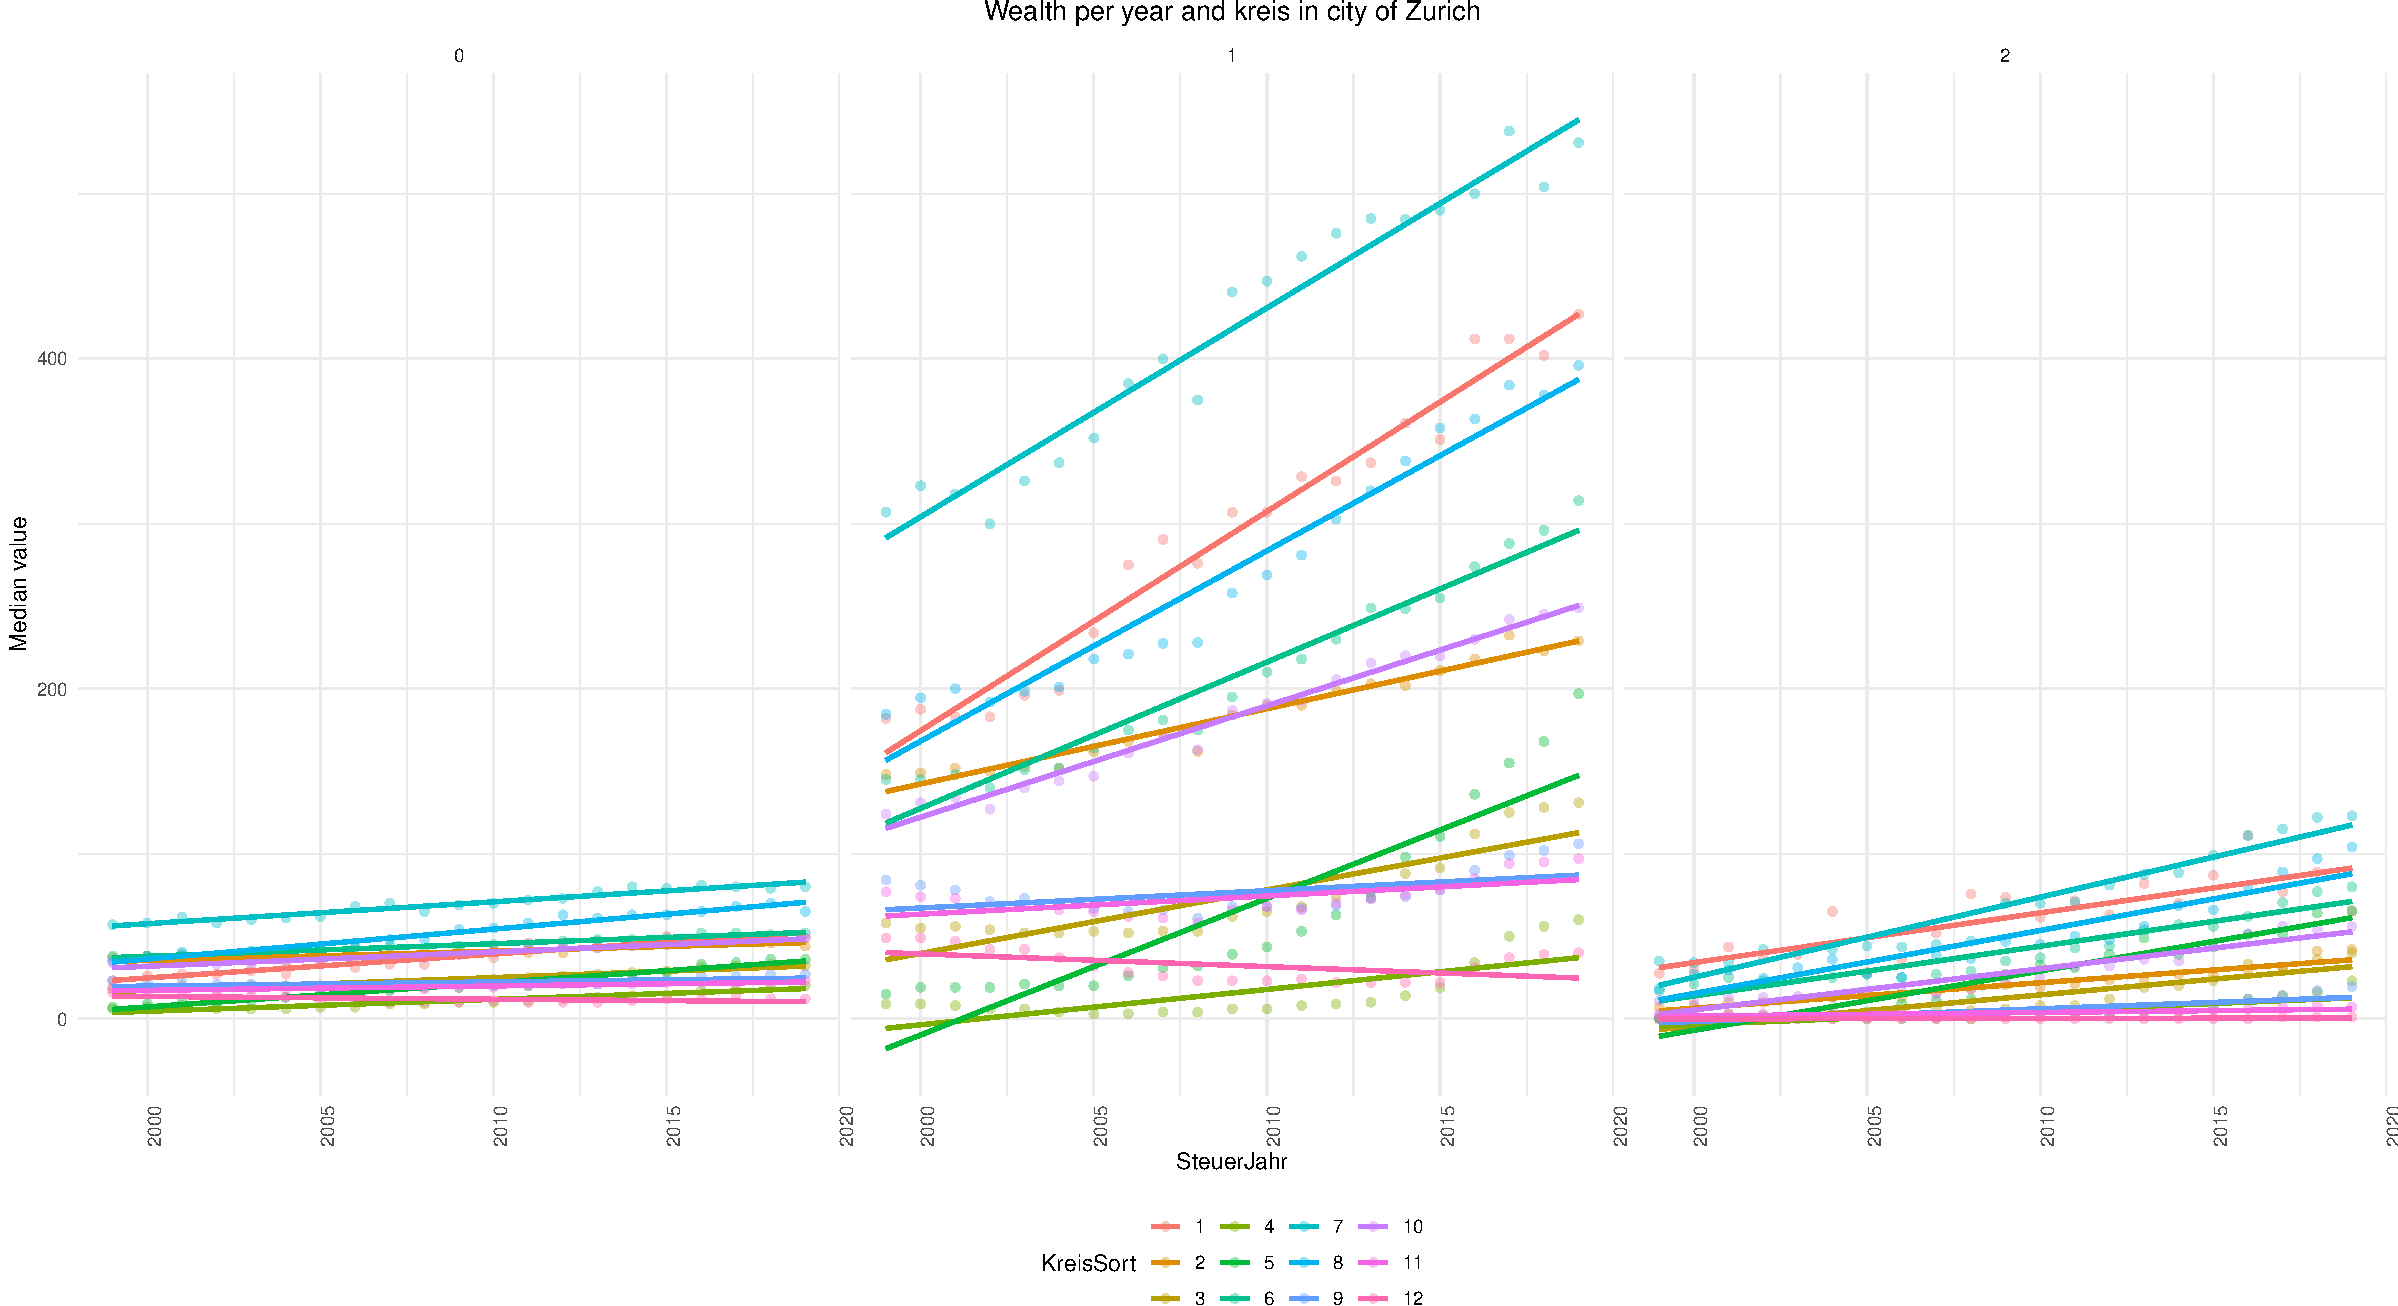
\includegraphics{report_files/figure-latex/plot_wealth-1.pdf}

\hypertarget{data-set-4-income-distribution-of-the-population-in-zuxfcrich-by-district}{%
\subsection{Data set 4: Income distribution of the population in Zürich,
by
district}\label{data-set-4-income-distribution-of-the-population-in-zuxfcrich-by-district}}

The following data set of dimensions 756x8 variables reflects how the
income distribution in absolute terms changed over time per district and
per tax class. The following table shows the accumulated income
distribution across all districts of the city of Zürich between the
years 1999 and 2019.

\begin{longtable}[]{@{}rrlrlrrr@{}}
\caption{Original data set: Distribution income tax per category,
district and year}\tabularnewline
\toprule
\begin{minipage}[b]{(\columnwidth - 7\tabcolsep) * \real{0.08}}\raggedleft
SteuerJahr\strut
\end{minipage} &
\begin{minipage}[b]{(\columnwidth - 7\tabcolsep) * \real{0.08}}\raggedleft
KreisSort\strut
\end{minipage} &
\begin{minipage}[b]{(\columnwidth - 7\tabcolsep) * \real{0.08}}\raggedright
KreisLang\strut
\end{minipage} &
\begin{minipage}[b]{(\columnwidth - 7\tabcolsep) * \real{0.12}}\raggedleft
SteuerTarifSort\strut
\end{minipage} &
\begin{minipage}[b]{(\columnwidth - 7\tabcolsep) * \real{0.18}}\raggedright
SteuerTarifLang\strut
\end{minipage} &
\begin{minipage}[b]{(\columnwidth - 7\tabcolsep) * \real{0.15}}\raggedleft
SteuerEinkommen\_p50\strut
\end{minipage} &
\begin{minipage}[b]{(\columnwidth - 7\tabcolsep) * \real{0.15}}\raggedleft
SteuerEinkommen\_p25\strut
\end{minipage} &
\begin{minipage}[b]{(\columnwidth - 7\tabcolsep) * \real{0.15}}\raggedleft
SteuerEinkommen\_p75\strut
\end{minipage}\tabularnewline
\midrule
\endfirsthead
\toprule
\begin{minipage}[b]{(\columnwidth - 7\tabcolsep) * \real{0.08}}\raggedleft
SteuerJahr\strut
\end{minipage} &
\begin{minipage}[b]{(\columnwidth - 7\tabcolsep) * \real{0.08}}\raggedleft
KreisSort\strut
\end{minipage} &
\begin{minipage}[b]{(\columnwidth - 7\tabcolsep) * \real{0.08}}\raggedright
KreisLang\strut
\end{minipage} &
\begin{minipage}[b]{(\columnwidth - 7\tabcolsep) * \real{0.12}}\raggedleft
SteuerTarifSort\strut
\end{minipage} &
\begin{minipage}[b]{(\columnwidth - 7\tabcolsep) * \real{0.18}}\raggedright
SteuerTarifLang\strut
\end{minipage} &
\begin{minipage}[b]{(\columnwidth - 7\tabcolsep) * \real{0.15}}\raggedleft
SteuerEinkommen\_p50\strut
\end{minipage} &
\begin{minipage}[b]{(\columnwidth - 7\tabcolsep) * \real{0.15}}\raggedleft
SteuerEinkommen\_p25\strut
\end{minipage} &
\begin{minipage}[b]{(\columnwidth - 7\tabcolsep) * \real{0.15}}\raggedleft
SteuerEinkommen\_p75\strut
\end{minipage}\tabularnewline
\midrule
\endhead
\begin{minipage}[t]{(\columnwidth - 7\tabcolsep) * \real{0.08}}\raggedleft
1999\strut
\end{minipage} &
\begin{minipage}[t]{(\columnwidth - 7\tabcolsep) * \real{0.08}}\raggedleft
1\strut
\end{minipage} &
\begin{minipage}[t]{(\columnwidth - 7\tabcolsep) * \real{0.08}}\raggedright
Kreis 1\strut
\end{minipage} &
\begin{minipage}[t]{(\columnwidth - 7\tabcolsep) * \real{0.12}}\raggedleft
0\strut
\end{minipage} &
\begin{minipage}[t]{(\columnwidth - 7\tabcolsep) * \real{0.18}}\raggedright
Grundtarif\strut
\end{minipage} &
\begin{minipage}[t]{(\columnwidth - 7\tabcolsep) * \real{0.15}}\raggedleft
37.8\strut
\end{minipage} &
\begin{minipage}[t]{(\columnwidth - 7\tabcolsep) * \real{0.15}}\raggedleft
17.40\strut
\end{minipage} &
\begin{minipage}[t]{(\columnwidth - 7\tabcolsep) * \real{0.15}}\raggedleft
64.80\strut
\end{minipage}\tabularnewline
\begin{minipage}[t]{(\columnwidth - 7\tabcolsep) * \real{0.08}}\raggedleft
1999\strut
\end{minipage} &
\begin{minipage}[t]{(\columnwidth - 7\tabcolsep) * \real{0.08}}\raggedleft
1\strut
\end{minipage} &
\begin{minipage}[t]{(\columnwidth - 7\tabcolsep) * \real{0.08}}\raggedright
Kreis 1\strut
\end{minipage} &
\begin{minipage}[t]{(\columnwidth - 7\tabcolsep) * \real{0.12}}\raggedleft
1\strut
\end{minipage} &
\begin{minipage}[t]{(\columnwidth - 7\tabcolsep) * \real{0.18}}\raggedright
Verheiratetentarif\strut
\end{minipage} &
\begin{minipage}[t]{(\columnwidth - 7\tabcolsep) * \real{0.15}}\raggedleft
83.4\strut
\end{minipage} &
\begin{minipage}[t]{(\columnwidth - 7\tabcolsep) * \real{0.15}}\raggedleft
52.00\strut
\end{minipage} &
\begin{minipage}[t]{(\columnwidth - 7\tabcolsep) * \real{0.15}}\raggedleft
130.20\strut
\end{minipage}\tabularnewline
\begin{minipage}[t]{(\columnwidth - 7\tabcolsep) * \real{0.08}}\raggedleft
1999\strut
\end{minipage} &
\begin{minipage}[t]{(\columnwidth - 7\tabcolsep) * \real{0.08}}\raggedleft
1\strut
\end{minipage} &
\begin{minipage}[t]{(\columnwidth - 7\tabcolsep) * \real{0.08}}\raggedright
Kreis 1\strut
\end{minipage} &
\begin{minipage}[t]{(\columnwidth - 7\tabcolsep) * \real{0.12}}\raggedleft
2\strut
\end{minipage} &
\begin{minipage}[t]{(\columnwidth - 7\tabcolsep) * \real{0.18}}\raggedright
Einelternfamilientarif\strut
\end{minipage} &
\begin{minipage}[t]{(\columnwidth - 7\tabcolsep) * \real{0.15}}\raggedleft
46.7\strut
\end{minipage} &
\begin{minipage}[t]{(\columnwidth - 7\tabcolsep) * \real{0.15}}\raggedleft
26.05\strut
\end{minipage} &
\begin{minipage}[t]{(\columnwidth - 7\tabcolsep) * \real{0.15}}\raggedleft
87.05\strut
\end{minipage}\tabularnewline
\begin{minipage}[t]{(\columnwidth - 7\tabcolsep) * \real{0.08}}\raggedleft
1999\strut
\end{minipage} &
\begin{minipage}[t]{(\columnwidth - 7\tabcolsep) * \real{0.08}}\raggedleft
2\strut
\end{minipage} &
\begin{minipage}[t]{(\columnwidth - 7\tabcolsep) * \real{0.08}}\raggedright
Kreis 2\strut
\end{minipage} &
\begin{minipage}[t]{(\columnwidth - 7\tabcolsep) * \real{0.12}}\raggedleft
0\strut
\end{minipage} &
\begin{minipage}[t]{(\columnwidth - 7\tabcolsep) * \real{0.18}}\raggedright
Grundtarif\strut
\end{minipage} &
\begin{minipage}[t]{(\columnwidth - 7\tabcolsep) * \real{0.15}}\raggedleft
37.9\strut
\end{minipage} &
\begin{minipage}[t]{(\columnwidth - 7\tabcolsep) * \real{0.15}}\raggedleft
19.90\strut
\end{minipage} &
\begin{minipage}[t]{(\columnwidth - 7\tabcolsep) * \real{0.15}}\raggedleft
58.20\strut
\end{minipage}\tabularnewline
\begin{minipage}[t]{(\columnwidth - 7\tabcolsep) * \real{0.08}}\raggedleft
1999\strut
\end{minipage} &
\begin{minipage}[t]{(\columnwidth - 7\tabcolsep) * \real{0.08}}\raggedleft
2\strut
\end{minipage} &
\begin{minipage}[t]{(\columnwidth - 7\tabcolsep) * \real{0.08}}\raggedright
Kreis 2\strut
\end{minipage} &
\begin{minipage}[t]{(\columnwidth - 7\tabcolsep) * \real{0.12}}\raggedleft
1\strut
\end{minipage} &
\begin{minipage}[t]{(\columnwidth - 7\tabcolsep) * \real{0.18}}\raggedright
Verheiratetentarif\strut
\end{minipage} &
\begin{minipage}[t]{(\columnwidth - 7\tabcolsep) * \real{0.15}}\raggedleft
69.7\strut
\end{minipage} &
\begin{minipage}[t]{(\columnwidth - 7\tabcolsep) * \real{0.15}}\raggedleft
49.10\strut
\end{minipage} &
\begin{minipage}[t]{(\columnwidth - 7\tabcolsep) * \real{0.15}}\raggedleft
101.40\strut
\end{minipage}\tabularnewline
\begin{minipage}[t]{(\columnwidth - 7\tabcolsep) * \real{0.08}}\raggedleft
1999\strut
\end{minipage} &
\begin{minipage}[t]{(\columnwidth - 7\tabcolsep) * \real{0.08}}\raggedleft
2\strut
\end{minipage} &
\begin{minipage}[t]{(\columnwidth - 7\tabcolsep) * \real{0.08}}\raggedright
Kreis 2\strut
\end{minipage} &
\begin{minipage}[t]{(\columnwidth - 7\tabcolsep) * \real{0.12}}\raggedleft
2\strut
\end{minipage} &
\begin{minipage}[t]{(\columnwidth - 7\tabcolsep) * \real{0.18}}\raggedright
Einelternfamilientarif\strut
\end{minipage} &
\begin{minipage}[t]{(\columnwidth - 7\tabcolsep) * \real{0.15}}\raggedleft
39.2\strut
\end{minipage} &
\begin{minipage}[t]{(\columnwidth - 7\tabcolsep) * \real{0.15}}\raggedleft
21.90\strut
\end{minipage} &
\begin{minipage}[t]{(\columnwidth - 7\tabcolsep) * \real{0.15}}\raggedleft
58.90\strut
\end{minipage}\tabularnewline
\bottomrule
\end{longtable}

Examining the previous showed data revealed that the data set contains a
lot of irrelevant information. For example, the columns
\emph{``KreisSort''} and \emph{``KreisLang''} are redundant, since the
first in simply the encoding of the second in number. The same applies
for the the columns \emph{``SteuerTarifSort''} and
\emph{``SteuerTarifLang''}, since the first here again, is the encoding
of the second in number.\\
However, the columns \emph{``KreisLang''} and \emph{``SteuerTarifLang''}
are not redundant and therefore, droped.

\begin{longtable}[]{@{}rlrrrr@{}}
\caption{Final data set: Distribution wealth tax per category, district
and year}\tabularnewline
\toprule
\begin{minipage}[b]{(\columnwidth - 5\tabcolsep) * \real{0.11}}\raggedleft
SteuerJahr\strut
\end{minipage} &
\begin{minipage}[b]{(\columnwidth - 5\tabcolsep) * \real{0.10}}\raggedright
KreisSort\strut
\end{minipage} &
\begin{minipage}[b]{(\columnwidth - 5\tabcolsep) * \real{0.16}}\raggedleft
SteuerTarifSort\strut
\end{minipage} &
\begin{minipage}[b]{(\columnwidth - 5\tabcolsep) * \real{0.21}}\raggedleft
SteuerEinkommen\_p50\strut
\end{minipage} &
\begin{minipage}[b]{(\columnwidth - 5\tabcolsep) * \real{0.21}}\raggedleft
SteuerEinkommen\_p25\strut
\end{minipage} &
\begin{minipage}[b]{(\columnwidth - 5\tabcolsep) * \real{0.21}}\raggedleft
SteuerEinkommen\_p75\strut
\end{minipage}\tabularnewline
\midrule
\endfirsthead
\toprule
\begin{minipage}[b]{(\columnwidth - 5\tabcolsep) * \real{0.11}}\raggedleft
SteuerJahr\strut
\end{minipage} &
\begin{minipage}[b]{(\columnwidth - 5\tabcolsep) * \real{0.10}}\raggedright
KreisSort\strut
\end{minipage} &
\begin{minipage}[b]{(\columnwidth - 5\tabcolsep) * \real{0.16}}\raggedleft
SteuerTarifSort\strut
\end{minipage} &
\begin{minipage}[b]{(\columnwidth - 5\tabcolsep) * \real{0.21}}\raggedleft
SteuerEinkommen\_p50\strut
\end{minipage} &
\begin{minipage}[b]{(\columnwidth - 5\tabcolsep) * \real{0.21}}\raggedleft
SteuerEinkommen\_p25\strut
\end{minipage} &
\begin{minipage}[b]{(\columnwidth - 5\tabcolsep) * \real{0.21}}\raggedleft
SteuerEinkommen\_p75\strut
\end{minipage}\tabularnewline
\midrule
\endhead
\begin{minipage}[t]{(\columnwidth - 5\tabcolsep) * \real{0.11}}\raggedleft
1999\strut
\end{minipage} &
\begin{minipage}[t]{(\columnwidth - 5\tabcolsep) * \real{0.10}}\raggedright
1\strut
\end{minipage} &
\begin{minipage}[t]{(\columnwidth - 5\tabcolsep) * \real{0.16}}\raggedleft
0\strut
\end{minipage} &
\begin{minipage}[t]{(\columnwidth - 5\tabcolsep) * \real{0.21}}\raggedleft
37.8\strut
\end{minipage} &
\begin{minipage}[t]{(\columnwidth - 5\tabcolsep) * \real{0.21}}\raggedleft
17.40\strut
\end{minipage} &
\begin{minipage}[t]{(\columnwidth - 5\tabcolsep) * \real{0.21}}\raggedleft
64.80\strut
\end{minipage}\tabularnewline
\begin{minipage}[t]{(\columnwidth - 5\tabcolsep) * \real{0.11}}\raggedleft
1999\strut
\end{minipage} &
\begin{minipage}[t]{(\columnwidth - 5\tabcolsep) * \real{0.10}}\raggedright
1\strut
\end{minipage} &
\begin{minipage}[t]{(\columnwidth - 5\tabcolsep) * \real{0.16}}\raggedleft
1\strut
\end{minipage} &
\begin{minipage}[t]{(\columnwidth - 5\tabcolsep) * \real{0.21}}\raggedleft
83.4\strut
\end{minipage} &
\begin{minipage}[t]{(\columnwidth - 5\tabcolsep) * \real{0.21}}\raggedleft
52.00\strut
\end{minipage} &
\begin{minipage}[t]{(\columnwidth - 5\tabcolsep) * \real{0.21}}\raggedleft
130.20\strut
\end{minipage}\tabularnewline
\begin{minipage}[t]{(\columnwidth - 5\tabcolsep) * \real{0.11}}\raggedleft
1999\strut
\end{minipage} &
\begin{minipage}[t]{(\columnwidth - 5\tabcolsep) * \real{0.10}}\raggedright
1\strut
\end{minipage} &
\begin{minipage}[t]{(\columnwidth - 5\tabcolsep) * \real{0.16}}\raggedleft
2\strut
\end{minipage} &
\begin{minipage}[t]{(\columnwidth - 5\tabcolsep) * \real{0.21}}\raggedleft
46.7\strut
\end{minipage} &
\begin{minipage}[t]{(\columnwidth - 5\tabcolsep) * \real{0.21}}\raggedleft
26.05\strut
\end{minipage} &
\begin{minipage}[t]{(\columnwidth - 5\tabcolsep) * \real{0.21}}\raggedleft
87.05\strut
\end{minipage}\tabularnewline
\begin{minipage}[t]{(\columnwidth - 5\tabcolsep) * \real{0.11}}\raggedleft
1999\strut
\end{minipage} &
\begin{minipage}[t]{(\columnwidth - 5\tabcolsep) * \real{0.10}}\raggedright
2\strut
\end{minipage} &
\begin{minipage}[t]{(\columnwidth - 5\tabcolsep) * \real{0.16}}\raggedleft
0\strut
\end{minipage} &
\begin{minipage}[t]{(\columnwidth - 5\tabcolsep) * \real{0.21}}\raggedleft
37.9\strut
\end{minipage} &
\begin{minipage}[t]{(\columnwidth - 5\tabcolsep) * \real{0.21}}\raggedleft
19.90\strut
\end{minipage} &
\begin{minipage}[t]{(\columnwidth - 5\tabcolsep) * \real{0.21}}\raggedleft
58.20\strut
\end{minipage}\tabularnewline
\begin{minipage}[t]{(\columnwidth - 5\tabcolsep) * \real{0.11}}\raggedleft
1999\strut
\end{minipage} &
\begin{minipage}[t]{(\columnwidth - 5\tabcolsep) * \real{0.10}}\raggedright
2\strut
\end{minipage} &
\begin{minipage}[t]{(\columnwidth - 5\tabcolsep) * \real{0.16}}\raggedleft
1\strut
\end{minipage} &
\begin{minipage}[t]{(\columnwidth - 5\tabcolsep) * \real{0.21}}\raggedleft
69.7\strut
\end{minipage} &
\begin{minipage}[t]{(\columnwidth - 5\tabcolsep) * \real{0.21}}\raggedleft
49.10\strut
\end{minipage} &
\begin{minipage}[t]{(\columnwidth - 5\tabcolsep) * \real{0.21}}\raggedleft
101.40\strut
\end{minipage}\tabularnewline
\begin{minipage}[t]{(\columnwidth - 5\tabcolsep) * \real{0.11}}\raggedleft
1999\strut
\end{minipage} &
\begin{minipage}[t]{(\columnwidth - 5\tabcolsep) * \real{0.10}}\raggedright
2\strut
\end{minipage} &
\begin{minipage}[t]{(\columnwidth - 5\tabcolsep) * \real{0.16}}\raggedleft
2\strut
\end{minipage} &
\begin{minipage}[t]{(\columnwidth - 5\tabcolsep) * \real{0.21}}\raggedleft
39.2\strut
\end{minipage} &
\begin{minipage}[t]{(\columnwidth - 5\tabcolsep) * \real{0.21}}\raggedleft
21.90\strut
\end{minipage} &
\begin{minipage}[t]{(\columnwidth - 5\tabcolsep) * \real{0.21}}\raggedleft
58.90\strut
\end{minipage}\tabularnewline
\bottomrule
\end{longtable}

The next graph shows the distribution of income per year, tax category
and district in Zurich.

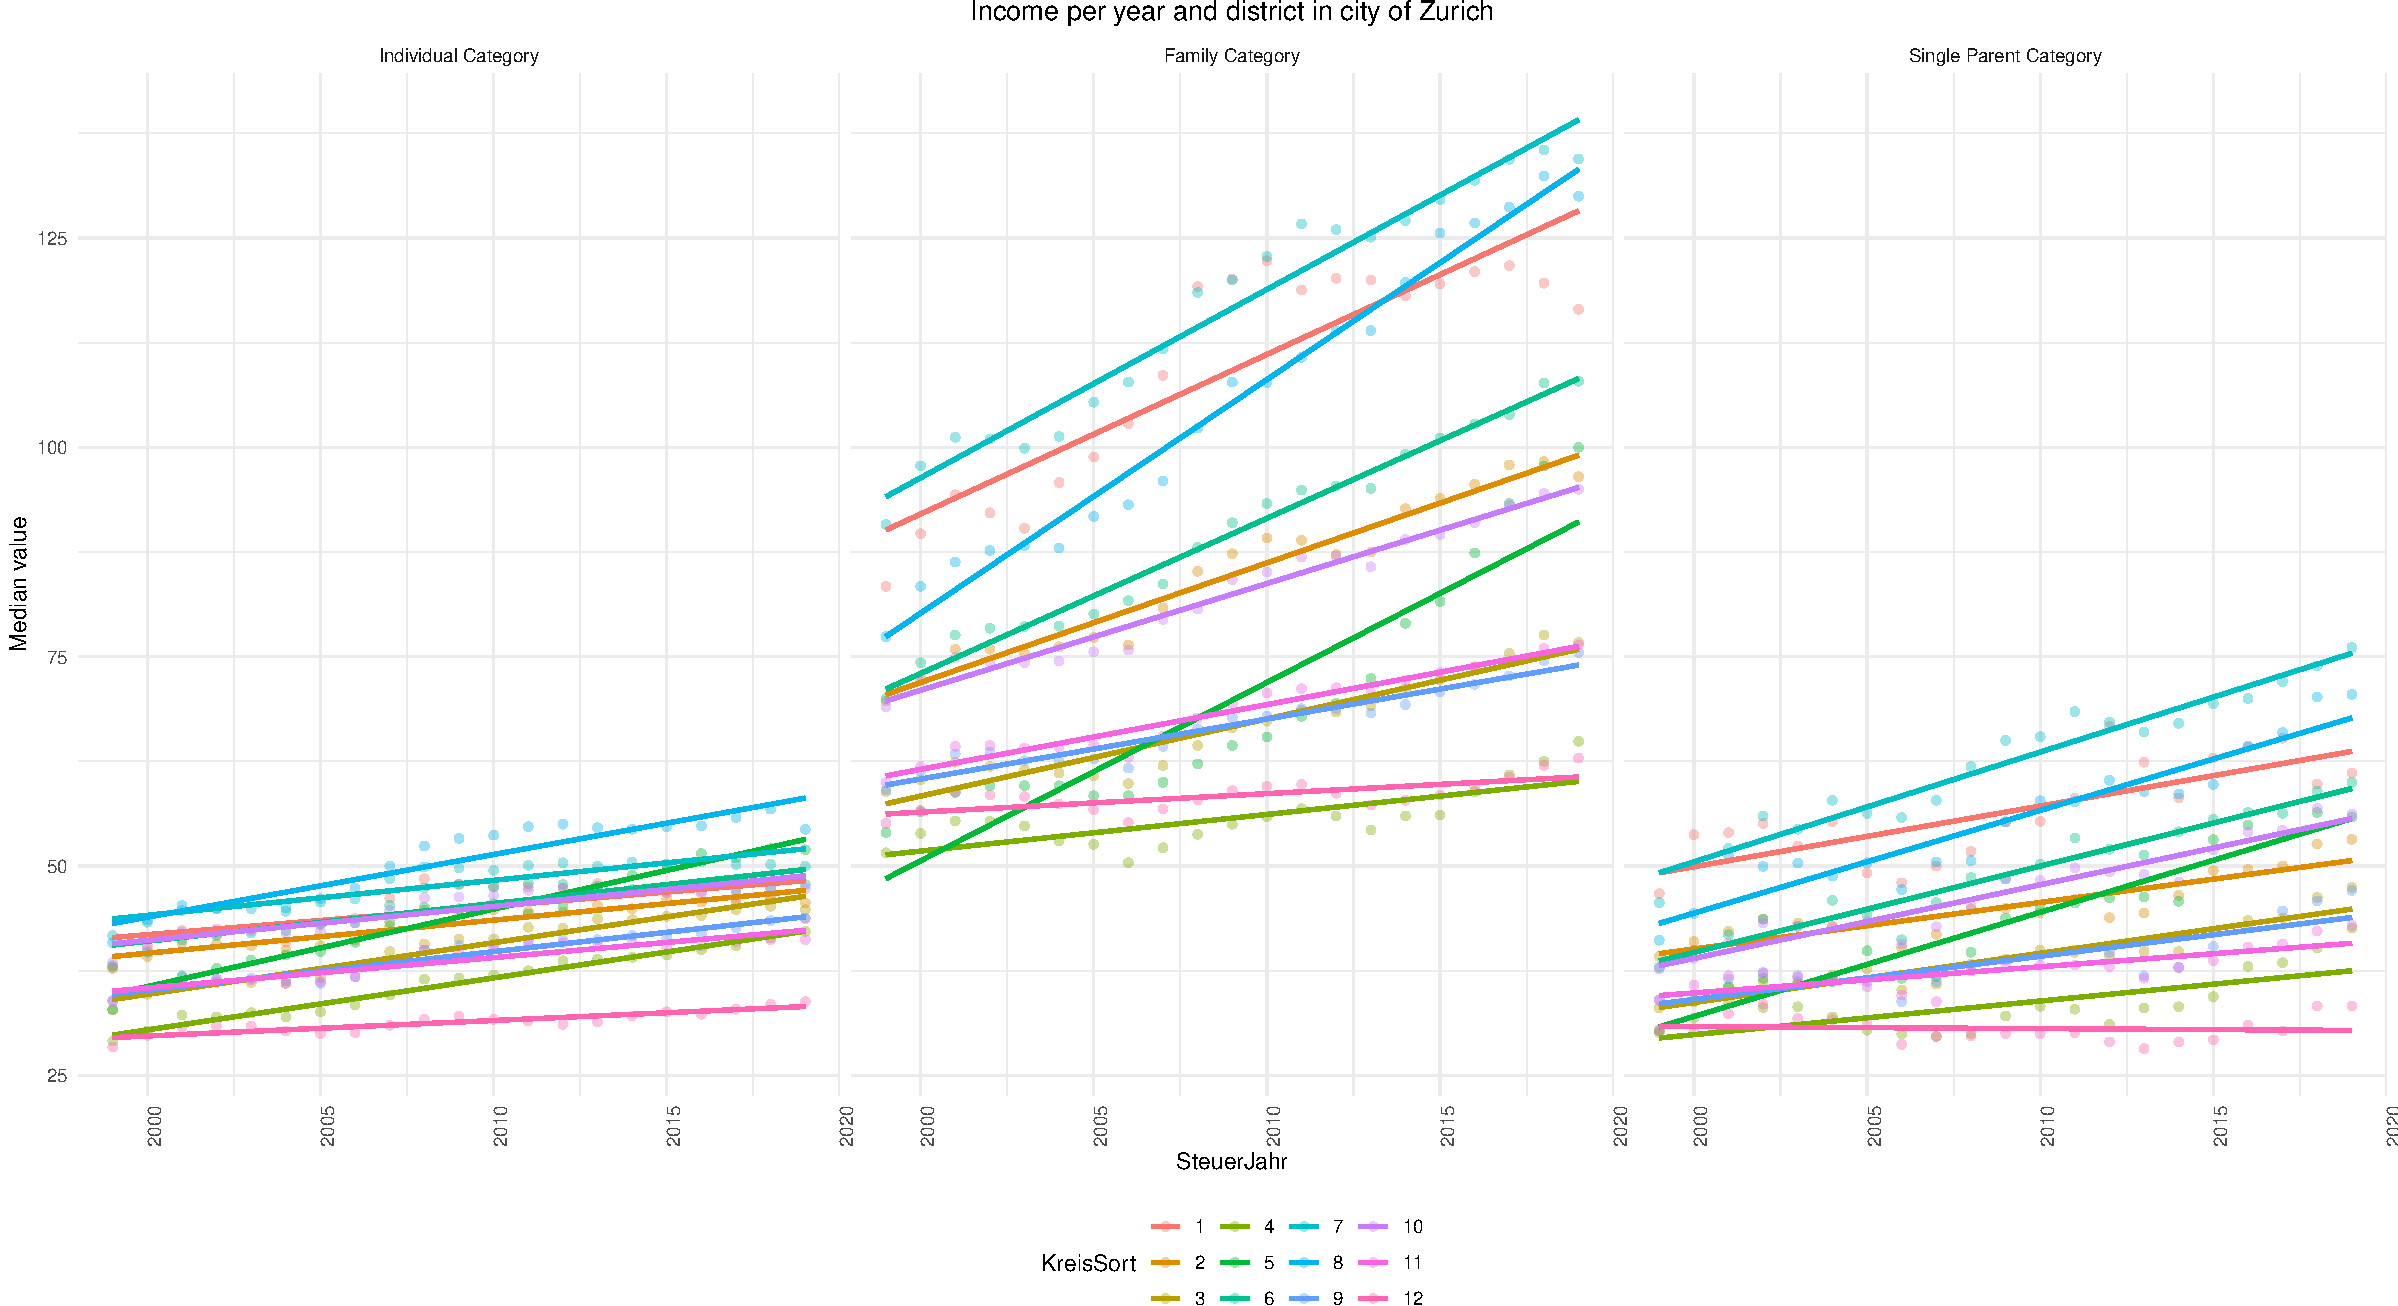
\includegraphics{report_files/figure-latex/plot_income-1.pdf}

\hypertarget{combine-wealth-and-income-data}{%
\subsection{Combine Wealth and Income
data}\label{combine-wealth-and-income-data}}

The aim of this part is to combine the income and wealth data into one
dataframe.

\begin{longtable}[]{@{}rlrrrrr@{}}
\caption{Merged income and wealth data}\tabularnewline
\toprule
\begin{minipage}[b]{(\columnwidth - 6\tabcolsep) * \real{0.09}}\raggedleft
SteuerJahr\strut
\end{minipage} &
\begin{minipage}[b]{(\columnwidth - 6\tabcolsep) * \real{0.09}}\raggedright
KreisSort\strut
\end{minipage} &
\begin{minipage}[b]{(\columnwidth - 6\tabcolsep) * \real{0.14}}\raggedleft
SteuerTarifSort\strut
\end{minipage} &
\begin{minipage}[b]{(\columnwidth - 6\tabcolsep) * \real{0.17}}\raggedleft
SteuerEinkommen\_p50\strut
\end{minipage} &
\begin{minipage}[b]{(\columnwidth - 6\tabcolsep) * \real{0.17}}\raggedleft
SteuerEinkommen\_p25\strut
\end{minipage} &
\begin{minipage}[b]{(\columnwidth - 6\tabcolsep) * \real{0.17}}\raggedleft
SteuerEinkommen\_p75\strut
\end{minipage} &
\begin{minipage}[b]{(\columnwidth - 6\tabcolsep) * \real{0.17}}\raggedleft
SteuerVermoegen\_p50\strut
\end{minipage}\tabularnewline
\midrule
\endfirsthead
\toprule
\begin{minipage}[b]{(\columnwidth - 6\tabcolsep) * \real{0.09}}\raggedleft
SteuerJahr\strut
\end{minipage} &
\begin{minipage}[b]{(\columnwidth - 6\tabcolsep) * \real{0.09}}\raggedright
KreisSort\strut
\end{minipage} &
\begin{minipage}[b]{(\columnwidth - 6\tabcolsep) * \real{0.14}}\raggedleft
SteuerTarifSort\strut
\end{minipage} &
\begin{minipage}[b]{(\columnwidth - 6\tabcolsep) * \real{0.17}}\raggedleft
SteuerEinkommen\_p50\strut
\end{minipage} &
\begin{minipage}[b]{(\columnwidth - 6\tabcolsep) * \real{0.17}}\raggedleft
SteuerEinkommen\_p25\strut
\end{minipage} &
\begin{minipage}[b]{(\columnwidth - 6\tabcolsep) * \real{0.17}}\raggedleft
SteuerEinkommen\_p75\strut
\end{minipage} &
\begin{minipage}[b]{(\columnwidth - 6\tabcolsep) * \real{0.17}}\raggedleft
SteuerVermoegen\_p50\strut
\end{minipage}\tabularnewline
\midrule
\endhead
\begin{minipage}[t]{(\columnwidth - 6\tabcolsep) * \real{0.09}}\raggedleft
1999\strut
\end{minipage} &
\begin{minipage}[t]{(\columnwidth - 6\tabcolsep) * \real{0.09}}\raggedright
1\strut
\end{minipage} &
\begin{minipage}[t]{(\columnwidth - 6\tabcolsep) * \real{0.14}}\raggedleft
0\strut
\end{minipage} &
\begin{minipage}[t]{(\columnwidth - 6\tabcolsep) * \real{0.17}}\raggedleft
37.8\strut
\end{minipage} &
\begin{minipage}[t]{(\columnwidth - 6\tabcolsep) * \real{0.17}}\raggedleft
17.40\strut
\end{minipage} &
\begin{minipage}[t]{(\columnwidth - 6\tabcolsep) * \real{0.17}}\raggedleft
64.80\strut
\end{minipage} &
\begin{minipage}[t]{(\columnwidth - 6\tabcolsep) * \real{0.17}}\raggedleft
23.0\strut
\end{minipage}\tabularnewline
\begin{minipage}[t]{(\columnwidth - 6\tabcolsep) * \real{0.09}}\raggedleft
1999\strut
\end{minipage} &
\begin{minipage}[t]{(\columnwidth - 6\tabcolsep) * \real{0.09}}\raggedright
1\strut
\end{minipage} &
\begin{minipage}[t]{(\columnwidth - 6\tabcolsep) * \real{0.14}}\raggedleft
1\strut
\end{minipage} &
\begin{minipage}[t]{(\columnwidth - 6\tabcolsep) * \real{0.17}}\raggedleft
83.4\strut
\end{minipage} &
\begin{minipage}[t]{(\columnwidth - 6\tabcolsep) * \real{0.17}}\raggedleft
52.00\strut
\end{minipage} &
\begin{minipage}[t]{(\columnwidth - 6\tabcolsep) * \real{0.17}}\raggedleft
130.20\strut
\end{minipage} &
\begin{minipage}[t]{(\columnwidth - 6\tabcolsep) * \real{0.17}}\raggedleft
182.0\strut
\end{minipage}\tabularnewline
\begin{minipage}[t]{(\columnwidth - 6\tabcolsep) * \real{0.09}}\raggedleft
1999\strut
\end{minipage} &
\begin{minipage}[t]{(\columnwidth - 6\tabcolsep) * \real{0.09}}\raggedright
1\strut
\end{minipage} &
\begin{minipage}[t]{(\columnwidth - 6\tabcolsep) * \real{0.14}}\raggedleft
2\strut
\end{minipage} &
\begin{minipage}[t]{(\columnwidth - 6\tabcolsep) * \real{0.17}}\raggedleft
46.7\strut
\end{minipage} &
\begin{minipage}[t]{(\columnwidth - 6\tabcolsep) * \real{0.17}}\raggedleft
26.05\strut
\end{minipage} &
\begin{minipage}[t]{(\columnwidth - 6\tabcolsep) * \real{0.17}}\raggedleft
87.05\strut
\end{minipage} &
\begin{minipage}[t]{(\columnwidth - 6\tabcolsep) * \real{0.17}}\raggedleft
27.5\strut
\end{minipage}\tabularnewline
\begin{minipage}[t]{(\columnwidth - 6\tabcolsep) * \real{0.09}}\raggedleft
1999\strut
\end{minipage} &
\begin{minipage}[t]{(\columnwidth - 6\tabcolsep) * \real{0.09}}\raggedright
10\strut
\end{minipage} &
\begin{minipage}[t]{(\columnwidth - 6\tabcolsep) * \real{0.14}}\raggedleft
0\strut
\end{minipage} &
\begin{minipage}[t]{(\columnwidth - 6\tabcolsep) * \real{0.17}}\raggedleft
38.5\strut
\end{minipage} &
\begin{minipage}[t]{(\columnwidth - 6\tabcolsep) * \real{0.17}}\raggedleft
20.00\strut
\end{minipage} &
\begin{minipage}[t]{(\columnwidth - 6\tabcolsep) * \real{0.17}}\raggedleft
57.30\strut
\end{minipage} &
\begin{minipage}[t]{(\columnwidth - 6\tabcolsep) * \real{0.17}}\raggedleft
34.0\strut
\end{minipage}\tabularnewline
\begin{minipage}[t]{(\columnwidth - 6\tabcolsep) * \real{0.09}}\raggedleft
1999\strut
\end{minipage} &
\begin{minipage}[t]{(\columnwidth - 6\tabcolsep) * \real{0.09}}\raggedright
10\strut
\end{minipage} &
\begin{minipage}[t]{(\columnwidth - 6\tabcolsep) * \real{0.14}}\raggedleft
1\strut
\end{minipage} &
\begin{minipage}[t]{(\columnwidth - 6\tabcolsep) * \real{0.17}}\raggedleft
69.0\strut
\end{minipage} &
\begin{minipage}[t]{(\columnwidth - 6\tabcolsep) * \real{0.17}}\raggedleft
49.60\strut
\end{minipage} &
\begin{minipage}[t]{(\columnwidth - 6\tabcolsep) * \real{0.17}}\raggedleft
98.40\strut
\end{minipage} &
\begin{minipage}[t]{(\columnwidth - 6\tabcolsep) * \real{0.17}}\raggedleft
124.0\strut
\end{minipage}\tabularnewline
\begin{minipage}[t]{(\columnwidth - 6\tabcolsep) * \real{0.09}}\raggedleft
1999\strut
\end{minipage} &
\begin{minipage}[t]{(\columnwidth - 6\tabcolsep) * \real{0.09}}\raggedright
10\strut
\end{minipage} &
\begin{minipage}[t]{(\columnwidth - 6\tabcolsep) * \real{0.14}}\raggedleft
2\strut
\end{minipage} &
\begin{minipage}[t]{(\columnwidth - 6\tabcolsep) * \real{0.17}}\raggedleft
37.7\strut
\end{minipage} &
\begin{minipage}[t]{(\columnwidth - 6\tabcolsep) * \real{0.17}}\raggedleft
20.65\strut
\end{minipage} &
\begin{minipage}[t]{(\columnwidth - 6\tabcolsep) * \real{0.17}}\raggedleft
54.15\strut
\end{minipage} &
\begin{minipage}[t]{(\columnwidth - 6\tabcolsep) * \real{0.17}}\raggedleft
11.0\strut
\end{minipage}\tabularnewline
\bottomrule
\end{longtable}

\pagebreak

\hypertarget{merging-data}{%
\section{Merging Data}\label{merging-data}}

\pagebreak

\hypertarget{data-visualization}{%
\section{Data Visualization}\label{data-visualization}}

\pagebreak

\hypertarget{fit-model}{%
\section{Fit Model}\label{fit-model}}

\pagebreak

\hypertarget{chapter-of-choice-tbd}{%
\section{Chapter of Choice TBD}\label{chapter-of-choice-tbd}}

\pagebreak

\hypertarget{references}{%
\section{References}\label{references}}

\end{document}
